\chapter{Eksperymenty badawcze}\label{chap:experiments}
Eksperymenty badawcze wyryfikujące charakterystyki sensorów, jak również dokładności opracowanej autorsko hybrydowej metody śledzenia ruchu kończyn, zostały wykonane w~laboratorium technik multimedialnych w~Centrum Technologii Informacyjnych Politechniki Łódzkiej. Jako źródło danych referencyjnych wykorzystany został zainstalowany tam system śledzenia ruchu firmy Vicon zbudowany na bazie 10 kamer Vicon T-40S \footfullcite{footnote:ViconSpec} rejestrujących ruch markerów. System ten został skonfigurowany do działania z~częstotliwością 100 klatek na sekundę, a~dane przetwarzane były przez dedykowaną aplikację Nexus w~wersji 2.0. Dane testowe niezbędne do zweryfikowania omawianej metody zostały zgromadzone przy użyciu kontrolera Microsoft Kinect w~wersji dla konsoli XBox 360 model 1414 oraz przez urządzenie rejestrujące dane z~czujników inercyjnych zaprojektowane i~wykonane samodzielnie. Szczegółowy opis przeprowadzonych eksperymentów badawczych znajduje się w~dalszej części niniejszej dysertacji.

\section{Scena}
Obszar roboczy, na którym dokonywane były pomiary ruchu, został zamknięty w~przestrzeni (prostopadłościanu) obserwowanej przez kamery systemu Vicon, której obrys podstawy zbliżony był do kwadratu $4m$x$4m$. W~trakcie kalibracji systemu referencyjnego punkt początkowy $\left(0, 0, 0\right)$ został zdefiniowany w~miejscu, w~którym został umieszczony kontroler Kinect. W~trakcie trwania eksperymentu, badany użytkownik stał w~odległości ok. $2m$ od Kinecta, czyli w~odległości, w~której działa on najbardziej dokładnie.  Pełne rozmieszczenie urządzeń na scenie prezentuje rysunek \ref{fig:experiments:scene}. Prostokąty dookoła obszaru roboczego oznaczone V1 -- V10 to kamery systemu Vicon.

\begin{savenotes}
	\begin{figure}[!htb]
		\centering
		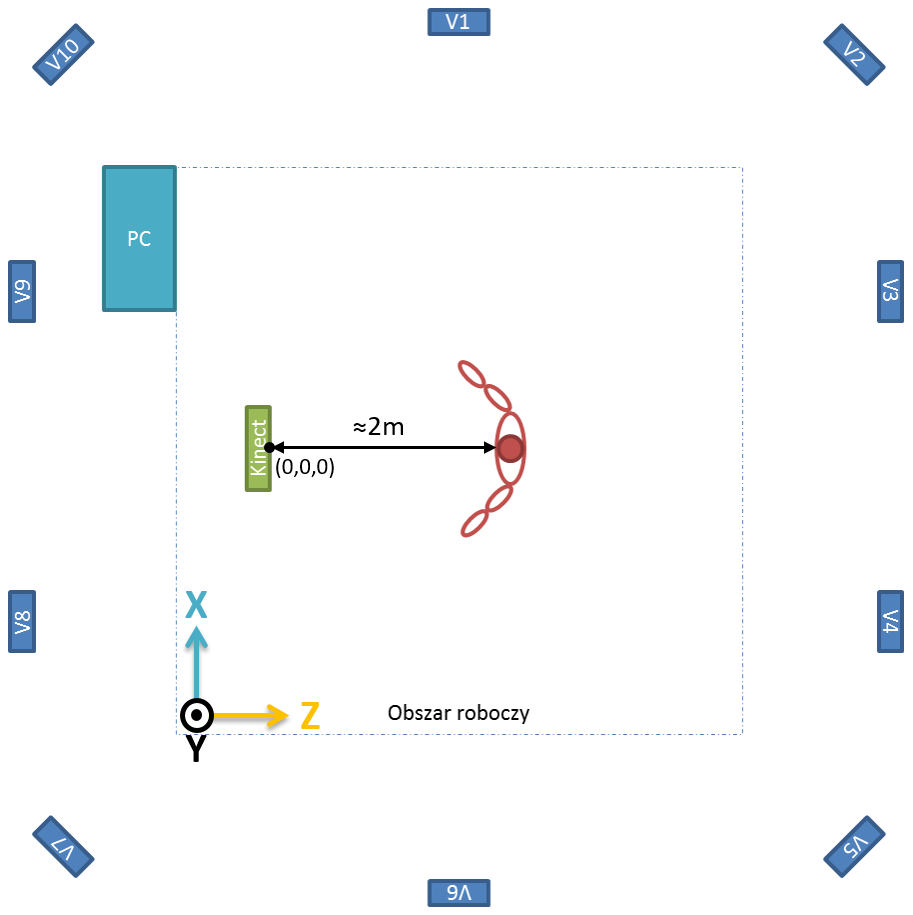
\includegraphics[width=0.7\textwidth]{images/scene.png}
		\caption{Schemat rozmieszczenia elementów sceny w~laboratorium}
		\label{fig:experiments:scene}
	\end{figure}
\end{savenotes}
		  
		 
Eksperymenty badawcze, opisane w~niniejszej pracy, zostały przeprowadzone na przykładzie ruchu ręki, a~oszacowaniu położenia w~przestrzeni podlega staw łokciowy oraz nadgarstkowy prawej ręki. Nie ogranicza to jednak możliwości zastosowania opracowanej w~pracy metody do śledzenia pozostałych kończyn. Markery niezbędne do prawidłowego działania systemu śledzenia ruchu firmy Vicon zostały umieszczone według schematu zamieszczonego na rysunku \ref{fig:experiments:viconArm}
		
\begin{savenotes}
	\begin{figure}[!htb]
		\centering
		\includegraphics[width=0.75\textwidth]{images/Fig11.png}
		\caption{Schemat romieszczenia markerów na ręce zgodny z~zaleceniami systemu Vicon}
		\label{fig:experiments:viconArm}
	\end{figure}
\end{savenotes}
				
Sposób umieszczenia markerów został zaczerpnięty ze schematu ich rozmieszczenia zawartego w~instrukcji do systemu Vicon, jednak poszerzony został o~dodatkowe markery tak, aby nadgarstek i~łokieć śledzony był za pomocą czterech znaczników, a~ramię za pomocą trzech. Aby móc skutecznie porównać ze sobą położenie stawów, wyznaczonych na podstawie pomiarów z~kontrolera Kinect i~z czujników inercyjnych, z~tymi wyznaczonymi przez system śledzenia ruchu Vicon, współrzędne śledzonych markerów, reprezentujące wybrany staw, muszą być uśrednione, tak żeby na ich podstawie obliczyć współrzędne stawów analizowanej kończyny. Do dokładnego wyznaczenia pojedynczego punktu reprezentującego staw, pomocne jest oszacowanie położenia trzech markerów. Dzięki zastosowaniu uzupełniających markerów do układu rekomendowanego przez firmę Vicon, udało się znacznie ograniczyć liczbę pomiarów, na których były widoczne mniej niż trzy markery, przez co precyzja śledzenia ruchu kończyn była większa. System śledzenia ruchu Vicon, w~wykorzystanej konfiguracji, dostarczał pomiary co 10 ms -- działał z~częstotliwością 100 Hz.  \\ 
%([NotFixed] można coś wspomnieć o~ksiązkowej dokładności tego systemu i~że może pracować z~wieksza częstotliwością tylko że nie jest to potrzebne) -- nie znalazłem nigdzie dokładności dla tego konkretnego modelu kamer\\
				
Oprócz markerów niezbędnych dla poprawnego działania systemu Vicon na przedramieniu i~ramieniu, w~połowie ich długości, zostały umieszczone czujniki inercyjne. Czujniki te, aby możliwie wiernie rejestrować ruchy kończyn zostały przymocowane do skóry za pomocą taśmy klejącej oraz dodatkowo dociśnięte elastycznymi opaskami. Dzięki temu były one w~stanie wykonywać obroty wraz z~kończynami minimalizując względne przesunięcia. Zostały one umieszczone na wierzchniej stronie ręki, tam gdzie jest relatywnie cienka warstwa mięśni i~ścięgien. Dzięki temu czujniki w~większym stopniu reagowały na obroty kości i~były mniej wrażliwe na pracę otaczających je tkanek (wpływ ruchu między innymi skóry, ścięgień i~mięśni na badanie ruchu kości można znaleźć w~\cite{Sati2016,Reinschmidt2016}).
				
\section{Badanie ruchu}
				
Każdy z~ruchów ręki był wykonany przez trzech aktorów i~wykonany w~dwóch seriach po pięć powtórzeń. Każda seria stanowiła osobną sesję śledzenia co oznacza, że każdy ruch został zarejestrowany w~sześciu sesjach (3 osoby po 2 sesje śledzenia na każde ćwiczenie). Podzielenie całego ćwiczenia na serie z~mniejszą liczbą powtórzeń związane było z~efektem zmęczenia aktorów, jakie było widoczne wraz z~kolejnymi powtórzeniami. Ćwiczenia jakie należało wykonać zostały dobrane w~taki sposób, aby sprawdzić opisaną metodę zarówno w~sytuacjach, w~których kontroler Kinect i~czujniki inercyjne działają w~uprzywilejowanym dla nich zakresie pracy jak i~w~takich, w~których jedno z~urządzeń posiada istotne ograniczenia w~działaniu. Wszystkie sekwencje rozpoczynały się od pozycji wyjściowej z~rękami rozłożonymi na boki w tak zwanej pozycji T (\emph{ang. T--pose}). Następnie, wykonywano zgięcie rąk w~łokciu ku górze (w płaszczyźnie XY) i~ich wyprostowanie w~celu zsynchronizowania pomiarów Kinecta i~czujników inercyjnych w~czasie. Po sekwencji synchronizującej następowały właściwe ćwiczenia, w~których każde powtórzenie zaczynało i~kończyło się pozycją T (\emph{ang. T--pose}). Wykonywane ćwiczenia prezentuje rysunek \ref{fig:experiments:poses}.
				
\begin{savenotes}
	\begin{figure}[!htb]
		\centering
		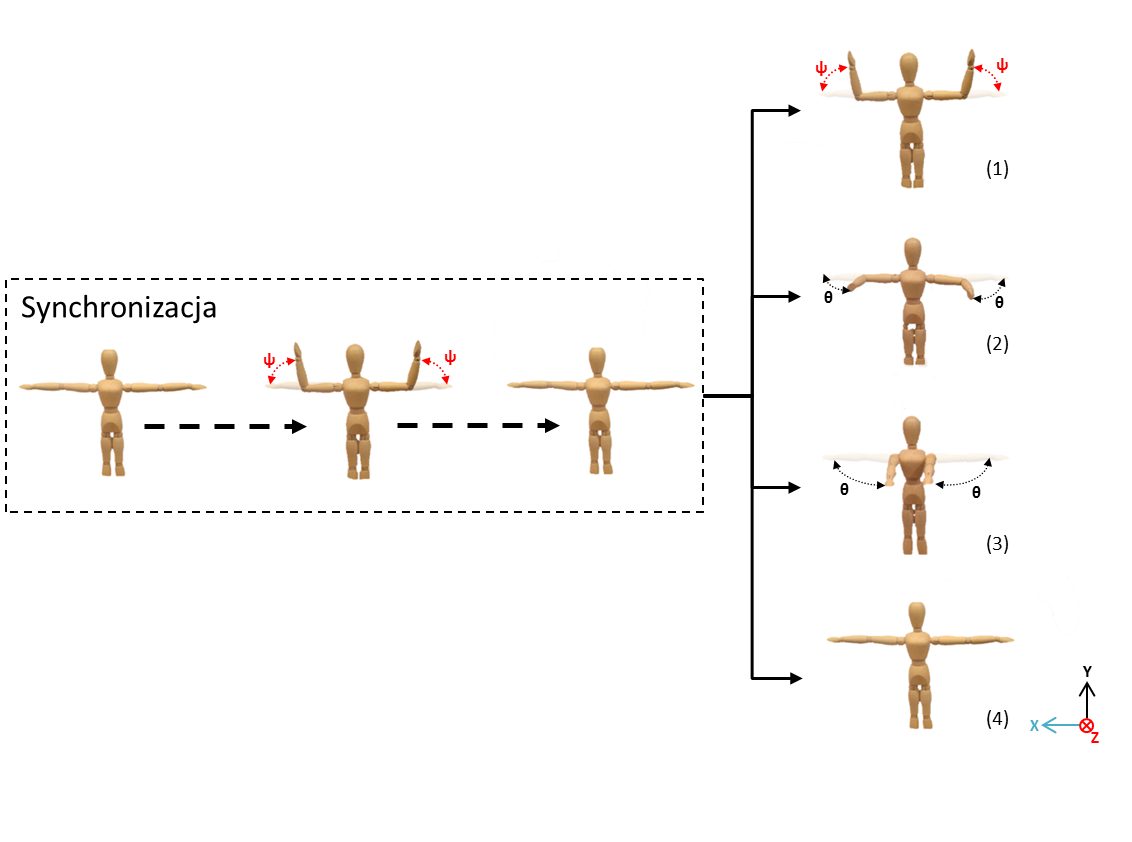
\includegraphics[width=\textwidth]{images/poses.png}
		\caption{Ćwiczenia wykonywane w~ramach eksperymentu}
		\label{fig:experiments:poses}
	\end{figure}
\end{savenotes}
						
Lista wykonywanych ćwiczeń obejmuje kolejno:
\begin{enumerate}
	\item Zgięcie ręki w~łokciu do góry (zgięcie w płaszczyźnie XY układu współrzędnych Kinecta); \\
	\item Zgięcie ręki w~łokciu do przodu (zgięcie w płaszczyźnie XZ układu współrzędnych Kinecta); \\
	\item Wyciągnięcie wyprostowanych ramion do przodu (ruch w płaszczyźnie XZ układu współrzędnych Kinecta); \\
	\item Utrzymanie wyprostowanych ramion w~bezruchu przez czas około 60s; \\
\end{enumerate}
						
Ćwiczenie 1 wykonywane było w~płaszczyźnie, w~której czujniki inercyjne są w~stanie dokonywać dokładnych i~stabilnych w~czasie pomiarów, natomiast dla Kinecta nie następuje okluzja stawów. Ćwiczenia 2 i~3 wymagają wykonania ruchu w~płaszczyźnie, w~której pomiary czujników inercyjnych są błędne i~nie mogą być traktowane jako wiarygodne. Dodatkowo, w~trakcie wykonywania ćwiczenia, kontroler Kinect traci możliwość obserwacji stawów ręki z~powodu ich przesłaniania się. Ostatnie ćwiczenie z~kolei sprawdza stabilność pomiaru w sytuacji kiedy nie jest wykonywany żaden ruch. Pomiar taki obarczony jest dryfem występującym w danych uzyskanych za pomocą akcelerometru i~żyroskopu.\\
						
Wszystkie pomiary zostały porównane z~pomiarami referencyjnymi zarejestrowanymi w~systemie Vicon w~celu określenia dokładności wyznaczania pozycji stawów i~kąta zgięcia w~łokciu. Układy współrzędnych systemu śledzenia Vicon i~systemu opartego na autorskiej metodzie śledzenia ruchu zostały ujednolicone tak aby można było łatwo określić precyzję szacowania położenia stawów. Jako główny przyjęto układ odniesienia systemu Vicon, w~którym punkt początkowy $(0,0,0)$ znajdował się na podłodze dokładnie pod kontrolerem Kinect.\\
						
Błąd estymacji pozycji stawów, w~pojedynczej sesji wykonywanego ruchu, został zdefiniowany jako pierwiastek kwadratowy z~błędu średniokwadratowego (RMSE -- \emph{ang. root mean square error}) odległości euklidesowej ($d_e()$) pomiędzy referencyjną pozycją danego stawu ($j$) zmierzoną w~systemie Vicon $P^V_j$, a~pozycją oszacowaną ($P^F_j$) i~jest wyrażony wzorem \ref{eq:experiments:RMSE}. Następnie została obliczona średnia arytmetyczna z~wyznaczonych błędów średniokwadratowych każdej z sesji śledzenia (wz. \ref{eq:experiments:average}), w~celu wyznaczenia dokładności szacowania pozycji stawów w~każdym z~wykonanych ćwiczeń. Podobną metodologię określania błędu oszacowania badanej metody zastosowali w~swoich pracach między innymi Kassim i in. \cite{Kassim2008} oraz Tadano i in. \cite{Tadano2013}. W~analogiczny sposób został także oszacowany błąd wyznaczania kąta zgięcia stawu łokciowego $\beta$.
						
\begin{equation}
	\centering
	RMSE^F_j = \sqrt{\frac{1}{n}\sum_{i=1}^{n}{d_e(P^V_{j,i}, P^F_{j,i})^2}}
	\label{eq:experiments:RMSE}
\end{equation}
						
Błędy szacowania pozycji stawów oraz kąta zgięcia stawu łokciowego zostały wyznaczone dla opisywanej w~niniejszej dysertacji metody łączenia danych, opartej na obrotach kości ($P^{F,O}_j$,$\beta^{F,O}$) oraz dla analogicznych oszacowań uzyskanych za pomocą metody o~najniższym opisanym w~literaturze błędzie szacowania położenia stawów -- metodzie Kalkbrenera i in. \cite{Kalkbrenner2014}. Metoda Kalkbrenera wykorzystuje  dane o pozycjach poszczególnych stawów, które są łączone celem zniwelowania niedokładności ($P^{F,P}_j$,$\beta^{F,P}$). \\
						
Każda z~sesji śledzenia konkretnego ruchu składała się z~5 nieprzerywanych powtórzeń tego samego ruchu. Dla każdej z~takich sesji zostały wyliczone wartości błędu średniokwadratowego każdego z~wyżej wymienionych oszacowań (pozycje stawów łokciowego ($P^F_E, j = E$  \emph{ang. Elbow}) i~nadgarstkowego ($P^F_W, j = W$ \emph{ang. Wrist}) oraz kąt zgięcia łokcia $\beta^F$). Całkowity błąd szacowania metody został określony jako średnia arytmetyczna błedów śrdniokwadratowych ($\overline{RMSE}$) ze wszystkich sześciu sesji śledzenia ruchu (indeks sesji śledzenia -- $s$) dla danego stawu (łokcia $E$ lub nadgarstka $W$) lub kąta $\beta$ (wz. \ref{eq:experiments:average}).
						
\begin{equation}
	\overline{RMSE^F_j} = \frac{\sum_{s=1}^{6}{RMSE^F_{j,s}}}{6}
	\label{eq:experiments:average}
\end{equation}
						
Wyniki zostały zebrane w~tabelach \ref{tab:experiments:first:avg}, \ref{tab:experiments:sec:avg}, \ref{tab:experiments:thr:avg} i~\ref{tab:experiments:four:avg}.
Porównanie pomiędzy wynikami uzyskanymi za pomocą metody Kalkbrennera i~metody łączenia danych opartej na obrotach kości zostało wyznaczone jako stosunek procentowy ($r$) różnicy pomiędzy uśrednionym błędem średniokwadratowym dla metody Kalkbrennera ($\overline{RMSE^P_j}$) a~uśrednonym błędem średniokwadratowym dla metody opracowanej przez autora niniejszej dysertacji ($\overline{RMSE^O_j}$) do $\overline{RMSE^P_j}$, gdzie $j$ oznacza analizowany staw szkieletu ($j=E, W$) lub kąt $\beta$. (wz. \ref{eq:experiments:comparison}). \\
						
\begin{equation}
	r = \frac{\overline{RMSE^P_j} - \overline{RMSE^O_j}}{\overline{RMSE^P_j}} * 100\%
	\label{eq:experiments:comparison}
\end{equation}
						
Dodatnia wartość $r$ oznacza, że uśredniony błąd średniokwadratowy wyników uzyskanych za pomocą metody opartej na łączeniu danych o obrotach jest mniejszy niż uśredniony błąd średniokwadratowy wyników uzyskanych metodą Kalkbrennera, co oznacza, że nastąpiła poprawa oszacowań. W przypadku wartości ujemnej mamy do czynienia z pogorszeniem uzyskiwanych wyników. W obu przypadkach wartość $r$ określa o ile procent zmieniły się wyniki. Porównanie uśrednionych błędów średniokwadratowych dla oszacowań:
\begin{itemize}
	\item położenia stawu łokciowego,
	\item położenia stawu nadgarstkowego,
	\item kąta zgięcia stawu łokciowego ($\beta$),
\end{itemize}
wykonanych za pomocą obu metod, zostało zaprezentowane na wykresach znajdujących się na rysunkach \ref{fig:experiments:elbow:summary}, \ref{fig:experiments:wrist:summary} oraz \ref{fig:experiments:angle:summary}.
						
\section*{Ćwiczenie 1 -- Zgięcie ramienia w~łokciu do góry}
Pierwsze ćwiczenie, jakie zostało wykonane z~użyciem omawianej metody, to zgięcie ręki w~łokciu do~góry (płaszczyzna XY układu odniesienia). Jest to ruch łatwy do śledzenia dla obu urządzeń pomiarowych ze względu na brak występowania okluzji stawów w płaszczyźnie ruchu prostopadłej do kierunku obserwacji Kinecta oraz ze względu na to, że nie odbywa się on wokół wektora grawitacji. Wyniki uzyskane w~tym ćwiczeniu prezentuje tabela \ref{tab:experiments:first:avg}.
						
\begin{table}[h]
	\caption[Średni błąd szacowania $\overline{RMSE}$ dla ćwiczenia nr 1]{Średni błąd szacowania $\overline{RMSE}$ (wz. \ref{eq:experiments:comparison})  dla ćwiczenia nr 1}
	\label{tab:experiments:first:avg}
	\noindent
	\tiny
	\centering
	\begin{tabular}{|c|N{1}{2}|N{1}{2}|N{1}{2}|N{1}{2}|N{1}{2}|N{1}{2}|}		
		\toprule 
		& \multicolumn{3}{c|}{{Metoda autorska}} & \multicolumn{3}{c|}{{Metoda Kalkbrennera}}  \\ 
		\midrule 
		{Sesja}                    & {$RMSE^O_E$} & {$RMSE^O_W$} & {$RMSE^O_\beta$} & {$RMSE^P_E$} & {$RMSE^P_W$} & {$RMSE^P_\beta$} \\
		{śledzenia}               & {$[cm]$}     & {$[cm]$}     & {$[\degree]$}    & {$[cm]$}     & {$[cm]$}     & {$[\degree]$}    \\	
		\midrule		
		1                          & 2.2498       & 2.7458       & 3.2398           & 2.6475       & 3.0934       & 3.4396           \\
		2                          & 2.2600       & 2.7635       & 3.3315           & 2.6598       & 3.1049       & 3.7705           \\
		3                          & 2.2308       & 2.7401       & 3.1499           & 2.5496       & 3.0193       & 3.4211           \\
		4                          & 2.2602       & 2.7603       & 3.1825           & 2.5593       & 3.0703       & 3.4827           \\
		5                          & 2.0592       & 2.7814       & 3.3570           & 2.4909       & 2.9371       & 3.5097           \\
		6                          & 2.2603       & 2.7718       & 3.5161           & 2.5602       & 2.9851       & 3.6250           \\
		\midrule
		Średnia $\overline{RMSE}$ & 2.2200       & 2.7605       & 3.2961           & 2.5779       & 3.0350       & 3.5414           \\
		Odchylenie                 & 0.0727       & 0.0141       & 0.1230           & 0.0585       & 0.0603       & 0.1216           \\
		\bottomrule
	\end{tabular} 																					
\end{table} 
						
Ćwiczenie polegające na wielokrotnym zgięciu ręki w~łokciu do góry, zgodnie z~przewidywaniami, dla obu urządzeń pomiarowych nie było trudne. Przez cały czas trwania ćwiczenia stawy były poprawnie identyfikowane i~w~pełni śledzone przez kontroler Kinect. Także czujniki inercyjne były w~stanie zarejestrować w~pełni  wykonywany ruch. Obie porównywane ze sobą metody łączące dane uzyskiwały podobne wyniki, a~zakres szacowanego przez nie ruchu był zbliżony do tego wykonywanego w rzeczywistości. Widoczne było natomiast zróżnicowanie w~dopasowaniu szkieletu do ciała ze względu na przyjęty model długości kości. W~metodzie Kalkbrennera miała miejsce częsta zmiana tego oszacowania, co wpływało na to, że śledzony staw potrafił zmienić swoje położenie podczas gdy postać pozostawała w bezruchu, a~także potrafił znaleźć się poza konturem postaci. W~przypadku metody autora niniejszej rozprawy, zauważalne były częste, jednak niewielkie, fluktuacje wartości oszacowanych pozycji stawów. Były one jednak na tyle niewielkie, że nie wpływały w istotny sposób na wartość błędu średniokwadratowego uzyskanego szacowania w przeciwieństwie do wpływu na ten błąd zmiennej długości segmentów reprezentujących kości wykorzystywanych w metodzie Kalkbrennera. Wydaje się również, że to właśnie brak stałego modelu długości kości w~metodzie Kalkbrennera ma największy wpływ na różnicę uzyskiwanych wyników w ćwiczeniu 1. \\
						
W omawianym ćwiczeniu ruch wykonywany był głównie przez przedramię, czyli istotne i~zamierzone zmiany położenia były widoczne na stawie nadgarstkowym. Wykresy \ref{fig:experiments:first:wristX}, \ref{fig:experiments:first:wristY}, \ref{fig:experiments:first:wristZ} pokazują położenie stawu nadgarstkowego w~każdej z~trzech osi w~trakcie wykonywania ruchu. Widać na nich wyraźną różnicę w~stabilności pomiarów objawiającą się ciągłymi drganiami widocznymi na wykresie łączenia danych za pomocą metody Kalkbrennera.
						
\begin{savenotes}
	\begin{figure}[!htb]
		\centering
		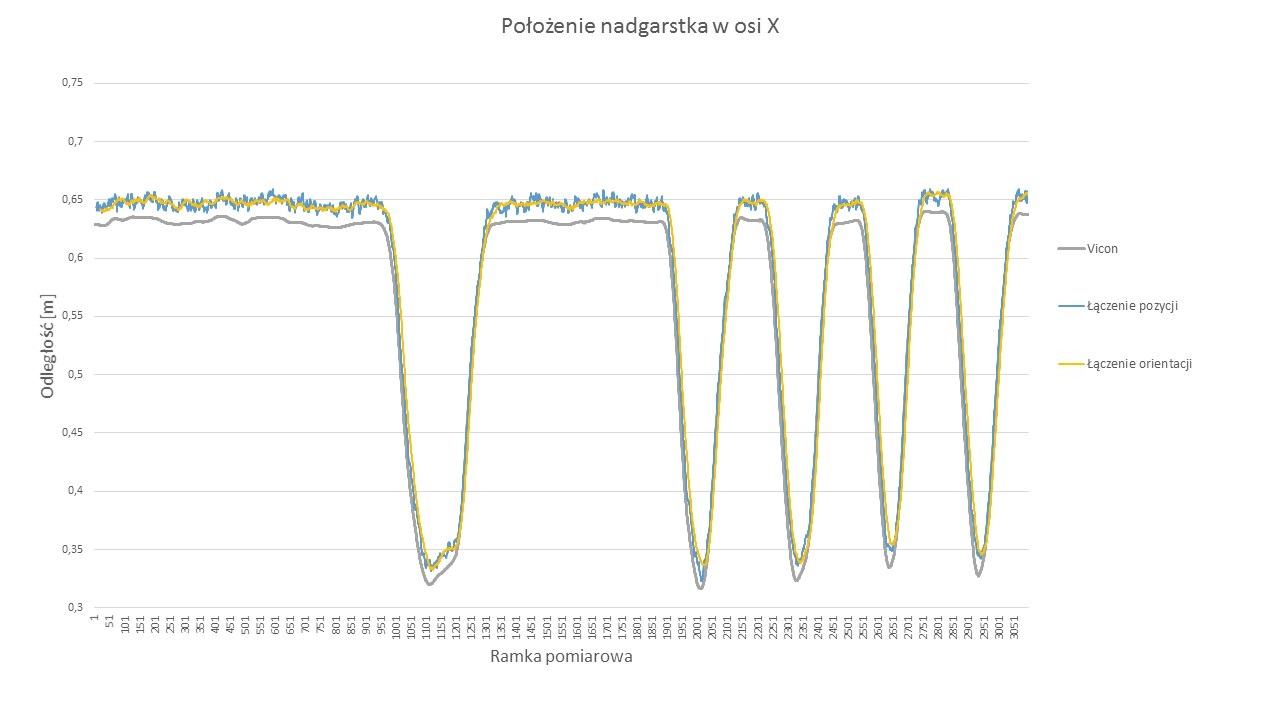
\includegraphics[width=0.9\linewidth]{images/100/Slide4.png}
		\caption{Wykres przedstawiający położenie stawu nadgarstkowego w~osi X}
		\label{fig:experiments:first:wristX}
	\end{figure}
\end{savenotes}
								
								
\begin{savenotes}
	\begin{figure}[!htb]
		\centering
		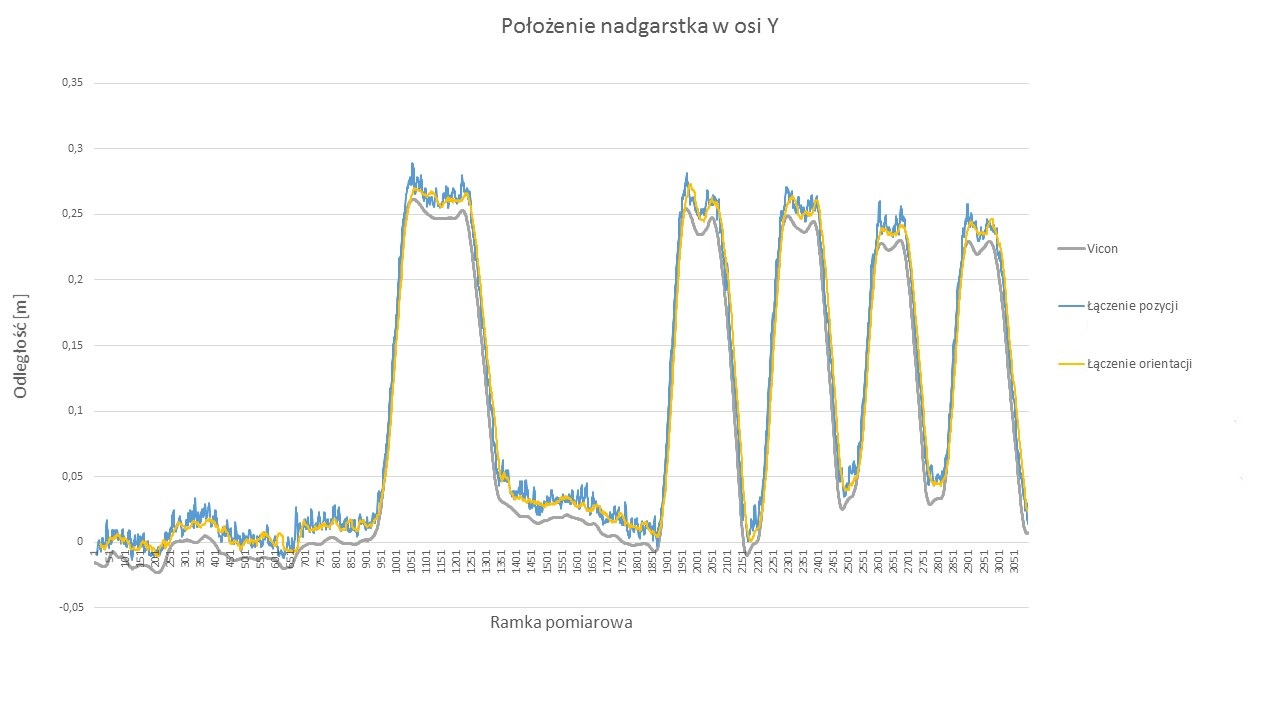
\includegraphics[width=0.9\linewidth]{images/100/Slide5.png}
		\caption{Wykres przedstawiający położenie stawu nadgarstkowego w~osi Y}
		\label{fig:experiments:first:wristY}
	\end{figure}
\end{savenotes}
										
\begin{savenotes}
	\begin{figure}[!htb]
		\centering
		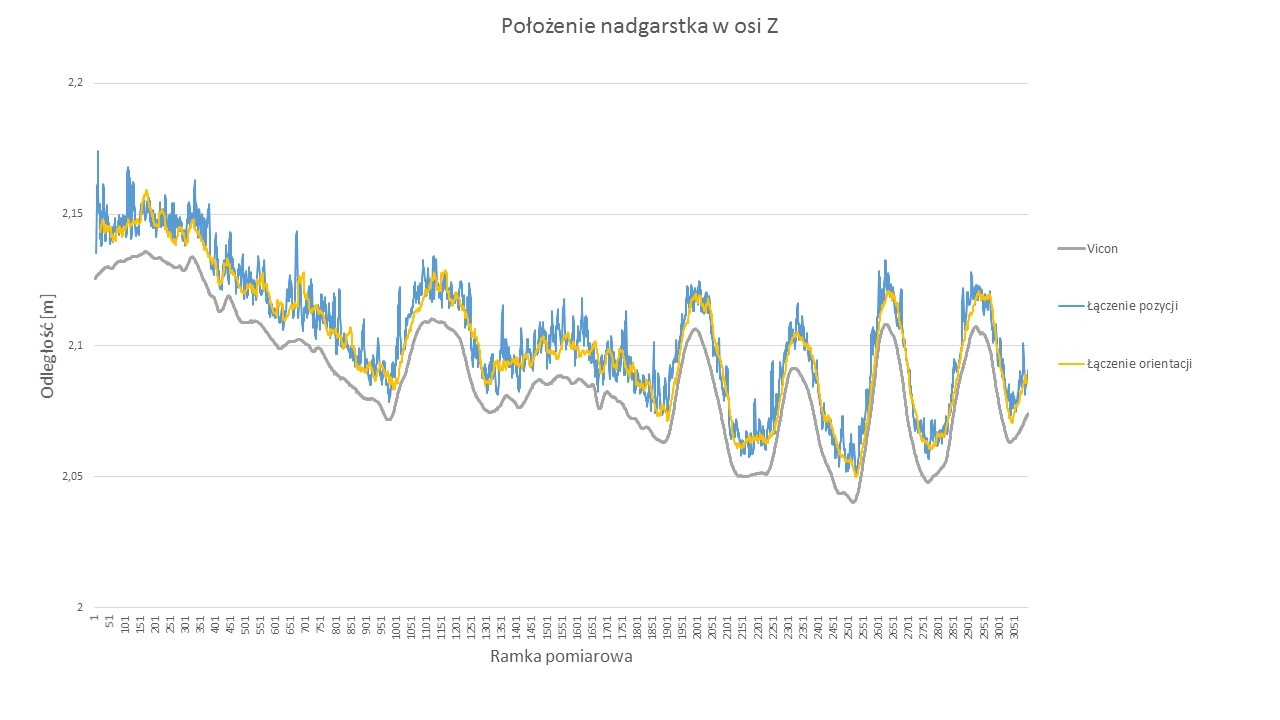
\includegraphics[width=0.9\linewidth]{images/100/Slide6.png}
		\caption{Wykres przedstawiający położenie stawu nadgarstkowego w~osi Z}
		\label{fig:experiments:first:wristZ}
	\end{figure}
\end{savenotes}
			
Wykres na rysunku \label{fig:experiments:first:angle} przedstawia oszacowanie kąta zgięcia ręki w łokciu ($\beta$). Widać na nim, wyraźną różnicę w dokładności i stabilności szacowania wartości w trakcie wykonywania ruchu oraz w położeniach skrajnych (wyprostowana ręka lub zgięta). W położeniu skrajnym widoczne są fluktuacje oszacowań zarówno za pomocą metody Kalkbrennera jak i metodą autorską. Jednakże fluktuacje obecne w oszacowaniach metody łączącej ze sobą obroty są widocznie mniejsze niż te występujące w metodzie opartej o łączenie pozycji stawów.
			
\begin{savenotes}
	\begin{figure}[!htb]
		\centering
		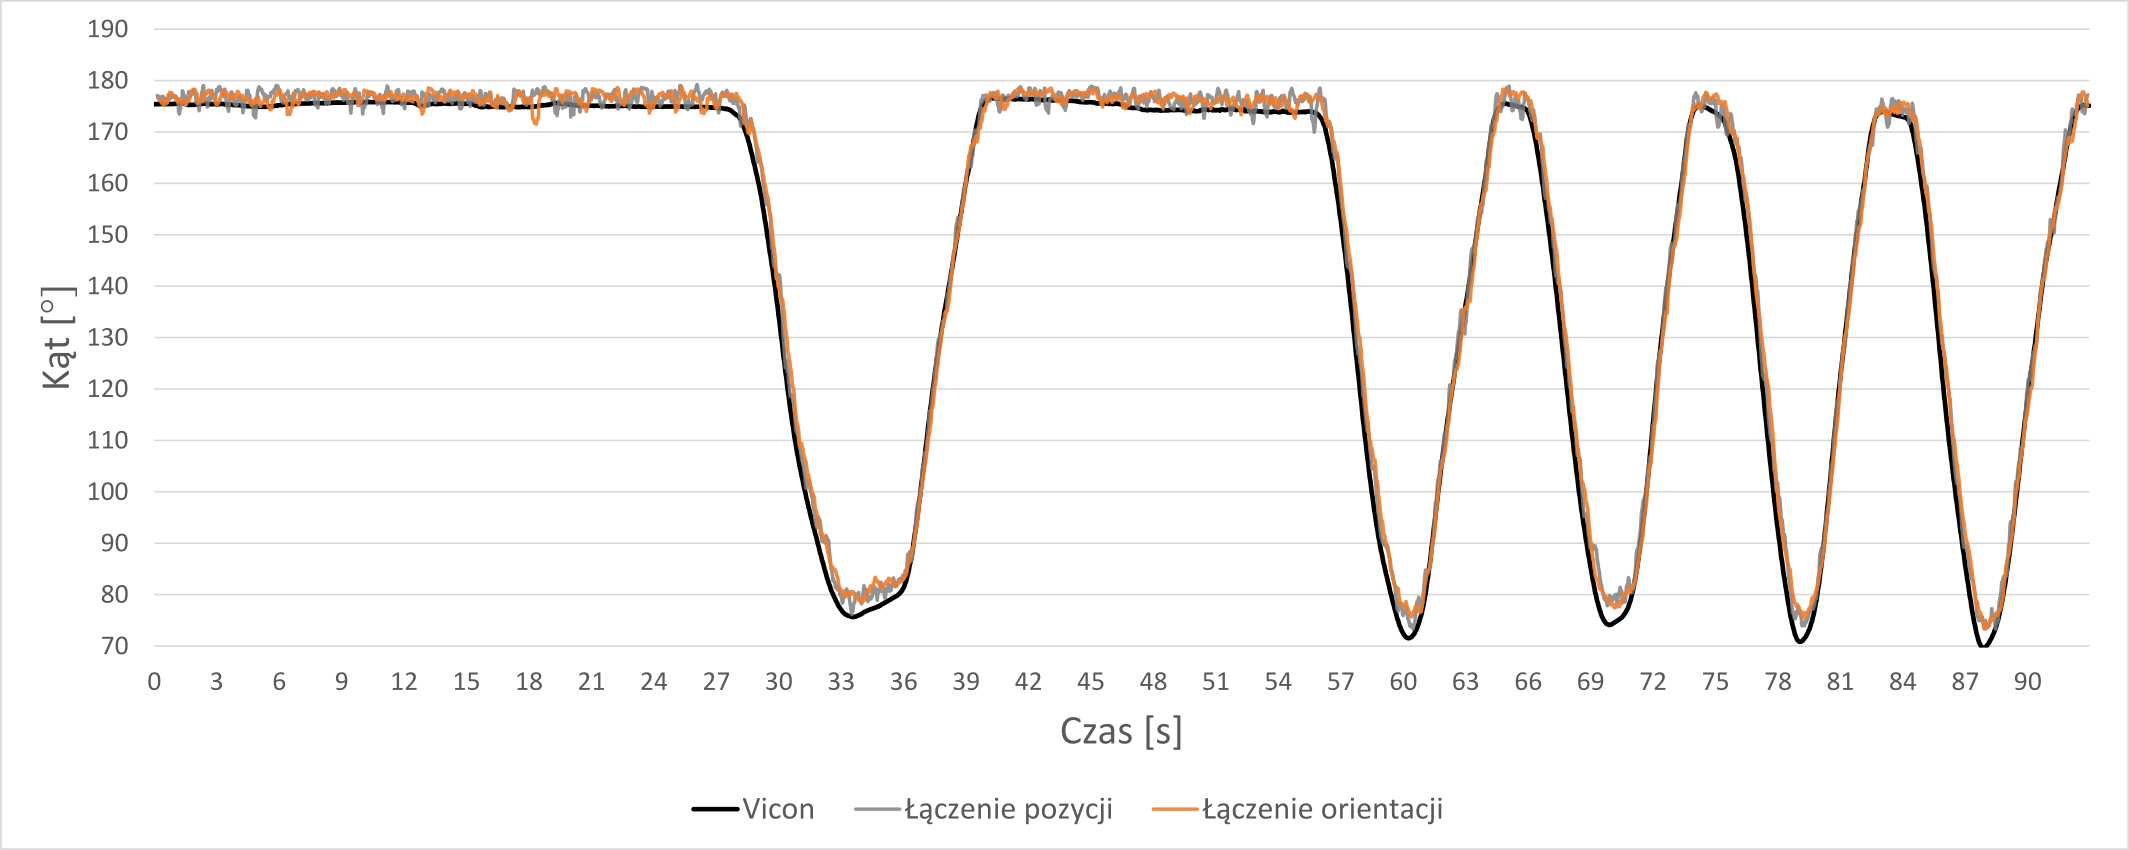
\includegraphics[width=0.9\linewidth]{images/100/angle.png}
		\caption{Wykres przedstawiający oszacowanie wartości kąta zgięcia ręki w łokciu ($\beta$) w trakcie ćwiczenia 1}
		\label{fig:experiments:first:angle}
	\end{figure}
\end{savenotes}
												
Rysunki \ref{fig:experiments:first:raw} oraz \ref{fig:experiments:first:fused} wizualizują ruch ręki podczas tego ćwiczenia. W~przypadku obu metod łączenia danych widać poprawę pozycjonowania stawów względem danych otrzymanych bezpośrednio z~urządzeń pomiarowych. 
												
\begin{savenotes}
	\begin{figure}[!htb]
		\captionsetup{singlelinecheck=off}
		\centering
		\begin{subfigure}[b]{0.65\textwidth}
			\centering
			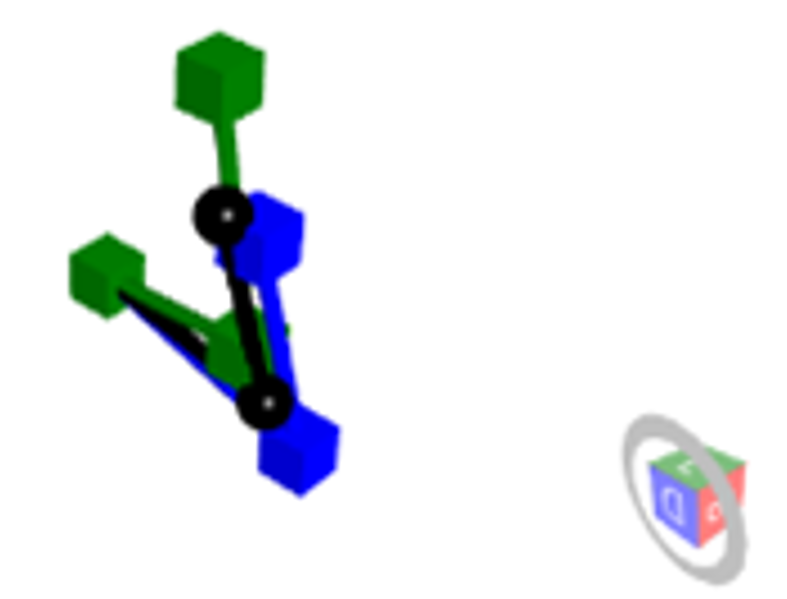
\includegraphics[width=\linewidth]{images/100/raw.png}	
			\caption{Wizualizacja ruchu bezpośrednio z~urządzeń pomiarowych}
			\label{fig:experiments:first:raw}
		\end{subfigure}
																																			
		\begin{subfigure}[b]{0.65\textwidth}
			\centering
			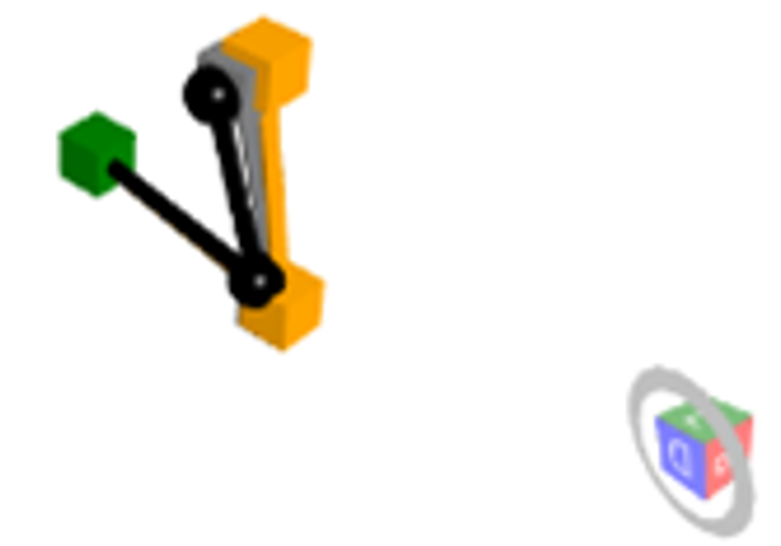
\includegraphics[width=\linewidth]{images/100/Fused.png}		
			\caption{Wizualizacja ruchu po złączeniu danych z~urządzeń pomiarowych}
			\label{fig:experiments:first:fused}	
		\end{subfigure}
																																		
		\caption[Wizualizacja ruchu ręki w~ćwiczeniu 1]{Wizualizacja ruchu ręki w~ćwiczeniu 1.  Kolory: czarny -- Vicon, niebieski -- czujniki inercyjne, zielony -- Kinect, szary -- metoda Kalkbrennera, pomarańczowy -- metoda autorska}	
		\label{fig:experiments:first}
	\end{figure}
\end{savenotes}
														
\section*{Ćwiczenia 2 i~3 -- Zgięcie ramienia w~łokciu do przodu oraz wyciągnięcie wyprostowanych ramion do przodu}
Ćwiczenia 2 i~3 przedstawiają ruchy o~zwiększonym stopniu trudności śledzenia dla obu urządzeń pomiarowych. W~tym przypadku następuje stopniowe przysłanianie jednego ze stawów co oznacza utratę możliwości dokładnego śledzenia ruchu przez kontroler Kinect. Dodatkowo ruch odbywał się w~płaszczyźnie trudnej z~punktu widzenia czujników inercyjnych, ponieważ obrót dokonywany był wokół osi równoległej do wektora grawitacji. Tabela \ref{tab:experiments:sec:avg} przedstawia średnie dokładności wykonywanego ruchu samego przedramienia, natomiast tabela \ref{tab:experiments:thr:avg} przedstawia wyniki dla ruchu całej wyprostowanej ręki.
														
\begin{table}[h]
	\caption[Średni błąd szacowania $\overline{RMSE}$ dla ćwiczenia nr 2]{Średni błąd szacowania $\overline{RMSE}$ (wz. \ref{eq:experiments:comparison}) dla ćwiczenia nr 2}
	\label{tab:experiments:sec:avg}
	\noindent
	\tiny
	\centering
	\begin{tabular}{|c|N{1}{2}|N{1}{2}|N{1}{2}|N{1}{2}|N{1}{2}|N{1}{2}|}		
		\toprule 
		& \multicolumn{3}{c|}{{Metoda autorska}} & \multicolumn{3}{c|}{{Metoda Kalkbrennera}}  \\ 
		\midrule 
		{Sesja}                    & {$RMSE^O_E$} & {$RMSE^O_W$} & {$RMSE^O_\beta$} & {$RMSE^P_E$} & {$RMSE^P_W$} & {$RMSE^P_\beta$} \\
		{śledzenia}               & {$[cm]$}     & {$[cm]$}     & {$[\degree]$}    & {$[cm]$}     & {$[cm]$}     & {$[\degree]$}    \\	
		\midrule		
		1                          & 2.6659       & 3.0214       & 14.4574          & 3.0815       & 3.4849       & 15.0134          \\
		2                          & 2.4977       & 2.8483       & 12.7191          & 3.0676       & 3.5101       & 13.0746          \\
		3                          & 2.3591       & 2.7377       & 12.7836          & 2.8575       & 3.2409       & 14.4970          \\
		4                          & 2.4143       & 2.9260       & 13.3775          & 3.1409       & 3.5275       & 15.2791          \\
		5                          & 2.4451       & 2.8774       & 13.4106          & 3.1591       & 3.4737       & 14.6086          \\
		6						   & 2.5134	      & 2.7932	     & 13,3402          & 2.9532	   & 3,5042	      & 14.5012			 \\		
		\midrule
		Średnia $\overline{RMSE}$ &2.4826    	  & 2.8673       & 13.3480          & 3.0613       & 3.4569       & 14.4957          \\
		Odchylenie                 & 0.1048       & 0.0931       & 0.6244           & 0.1075       & 0.1049       & 0.7634           \\
		\bottomrule
	\end{tabular} 
																																				
\end{table} 
														
\begin{table}[h]
	\caption[Średni błąd szacowania $\overline{RMSE}$ dla ćwiczenia nr 3]{Średni błąd szacowania $\overline{RMSE}$ (wz. \ref{eq:experiments:comparison}) dla ćwiczenia nr 3}
	\label{tab:experiments:thr:avg}
	\noindent
	\tiny
	\centering
	\begin{tabular}{|c|N{1}{2}|N{1}{2}|N{1}{2}|N{1}{2}|N{1}{2}|N{1}{2}|}		
		\toprule 
		& \multicolumn{3}{c|}{{Metoda autorska}} & \multicolumn{3}{c|}{{Metoda Kalkbrennera}}  \\ 
		\midrule 
		{Sesja}                    & {$RMSE^O_E$} & {$RMSE^O_W$} & {$RMSE^O_\beta$} & {$RMSE^P_E$} & {$RMSE^P_W$} & {$RMSE^P_\beta$} \\
		{śledzenia}               & {$[cm]$}     & {$[cm]$}     & {$[\degree]$}    & {$[cm]$}     & {$[cm]$}     & {$[\degree]$}    \\	
		\midrule		
		1                          & 2.5959       & 2.9683       & 13.3184          & 3.1288       & 3.5589       & 15.7465          \\
		2                          & 2.2391       & 2.5266       & 12.3694          & 2.9860       & 3.3287       & 13.1241          \\
		3                          & 2.7619       & 3.1413       & 13.1813          & 2.7030       & 3.1432       & 12.5385          \\
		4                          & 2.7347       & 3.0278       & 14.7809          & 3.1662       & 3.5129       & 16.4055          \\
		5                          & 2.2166       & 2.5777       & 16.7666          & 2.7412       & 3.0710       & 15.7460          \\
		6						   & 2.1975		  & 2.6912		 & 13.4102 			& 2.7532	   & 2.9042	      & 14.6612			\\
		\midrule																		
		Średnia $\overline{RMSE}$  & 2.4576	  	  & 2.8222  	 & 13.9711 	        & 2.9131	   & 3.2531		  & 14.7036	          \\
		Odchylenie                 & 0.2456		  & 0.2344  	 & 1.4376		    & 0.1893	   & 0.2358  	  & 1.4291           \\
		\bottomrule
	\end{tabular} 
																																				
\end{table} 
														
W obu ćwiczeniach, w~trakcie wykonywania ruchu, następował moment, w~którym jeden lub dwa stawy stawały się niewidoczne dla kontrolera Kinect, a~co za tym idzie, obie metody musiały bazować tylko na jednym źródle danych. Metoda opracowana przez autora niniejszej pracy nie wykorzystywała  w~trakcie łączenia danych pomiarów uzyskanych z~niepewnego źródła i~stopniowo wstrzymywała aktualizację estymowanego położenia stawu. Natomiast metoda Kalkbrennera wykorzystywała w~dalszym ciągu dane z~kontrolera Kinect zmieniając jedynie ich stopień istotności (rys. \ref{fig:experiments:sec:follow}). 
														
Ze względu na to, że kontroler Kinect, pomimo utraty możliwości śledzenia dowolnego stawu, wciąż estymuje jego położenie, zasadne jest sprawdzanie czy fuzja pomiarów dostarczonych przez kontroler Kinect z~pomiarami urządzeń inercyjnych nie sprawi, że ostateczna estymacja położenia stawu stanie się zbyt niedokładna. Metoda Kalkbrennera co prawda dokonuje takiego sprawdzenia w~trakcie stosowania filtru Kalmana, jednak widoczne było podążanie szacunkowych wartości położenia stawu za skokami danych z~Kinecta. Oznacza to, że wpływ pomiarów kontrolera Kinect na ostateczną estymację jest znaczący i~zastosowana w~metodzie Kalkbrennera zmiana stopnia ich istotności, w~procesie łączenia danych, jest niewystarczająca na ograniczenie negatywnego wpływu niedokładności kontrolera Kinect.
														
\begin{savenotes}
	\begin{figure}[!htb]
		\centering
		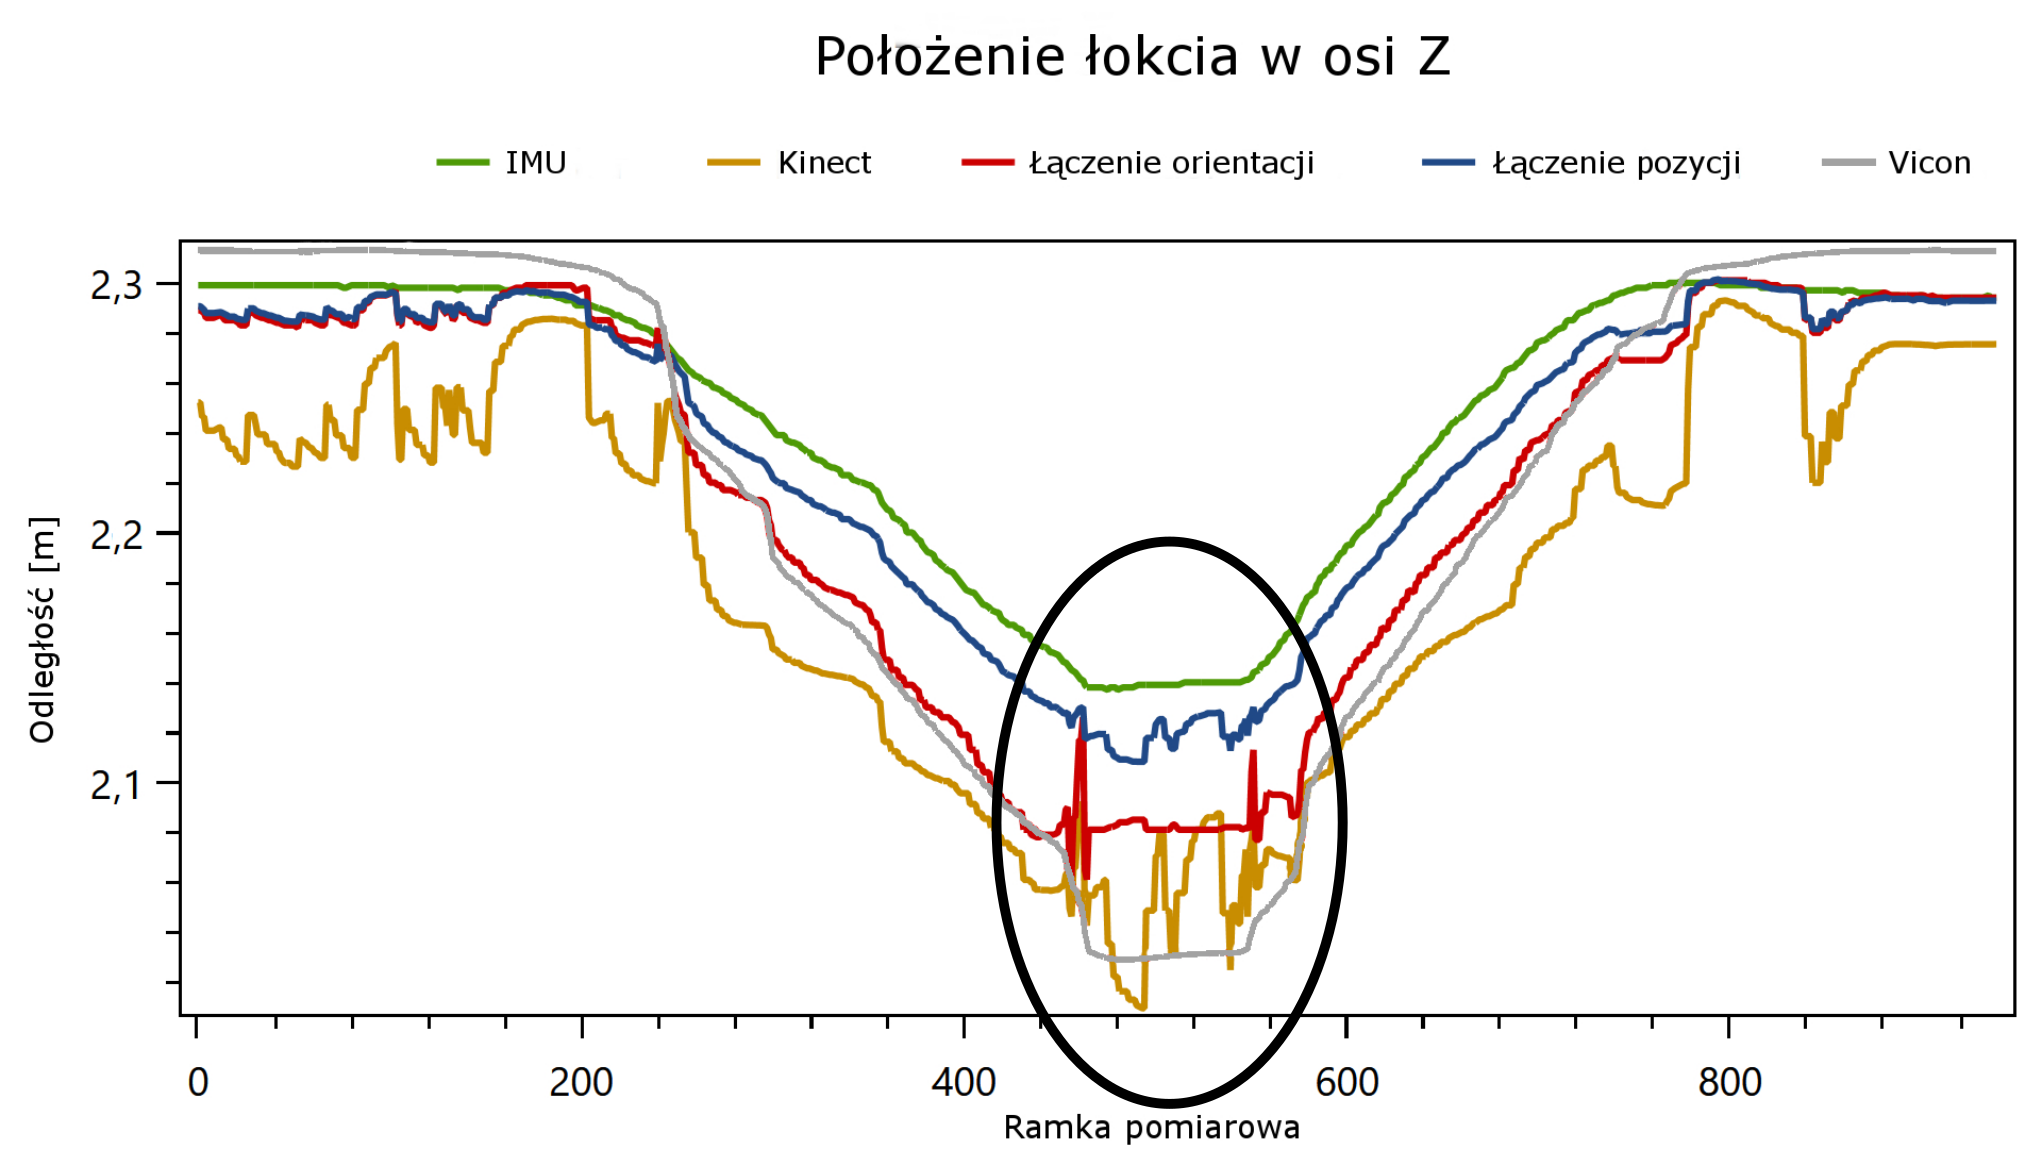
\includegraphics[width=0.9\linewidth]{images/300/Slide3_focus.png}
		\caption{Wykres przedstawiający podążanie wyznaczania pozycji stawu za pomiarami Kinecta w~trakcie wykonywania ćwiczenia 3}
		\label{fig:experiments:sec:follow}
	\end{figure}
\end{savenotes}
																
\begin{savenotes}
	\begin{figure}[!htb]
		\captionsetup{singlelinecheck=off}
		\centering
		\begin{subfigure}[b]{0.9\textwidth}
			\centering
			\includegraphics[width=\linewidth]{images/200/raw.png}	
			\caption{Wizualizacja ruchu bezpośrednio z~urządzeń pomiarowych}
			\label{fig:experiments:sec:raw}
		\end{subfigure}
																																							
		\begin{subfigure}[b]{0.9\textwidth}
			\centering
			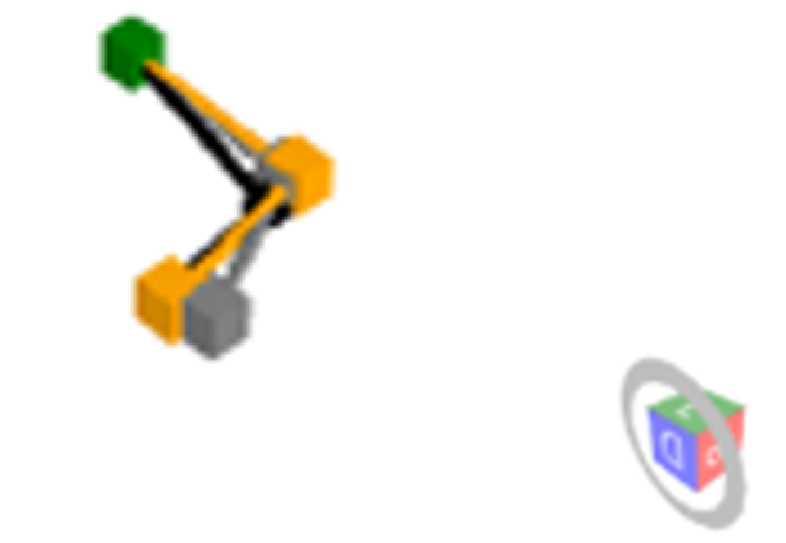
\includegraphics[width=\linewidth]{images/200/Fused.png}		
			\caption{Wizualizacja ruchu po złączeniu danych z~urządzeń pomiarowych}
			\label{fig:experiments:sec:fused}
		\end{subfigure}
																																						
		\caption[Wizualizacja ruchu ręki w~ćwiczeniu 2]{Wizualizacja ruchu ręki w~ćwiczeniu 2.  Kolory: czarny -- Vicon, niebieski -- czujniki inercyjne, zielony -- Kinect, szary -- metoda Kalkbrennera, pomarańczowy -- metoda autorska}	
		\label{fig:experiments:sec}
	\end{figure}
\end{savenotes}
%[Fixed]zlikwidować takie wypunktowanie w~podpisie rysunku. 
\begin{savenotes}
	\begin{figure}[!htb]
		\captionsetup{singlelinecheck=off}
		\centering
		\begin{subfigure}[b]{0.9\textwidth}
			\centering
			\includegraphics[width=\linewidth]{images/300/raw.png}	
			\caption{Wizualizacja ruchu bezpośrednio z~urządzeń pomiarowych}
			\label{fig:experiments:th:raw}
		\end{subfigure}
																																									
		\begin{subfigure}[b]{0.9\textwidth}
			\centering
			\includegraphics[width=\linewidth]{images/300/Fused.png}		
			\caption{Wizualizacja ruchu po złączeniu danych z~urządzeń pomiarowych}
			\label{fig:experiments:th:fused}	
		\end{subfigure}
																																								
		\caption[Wizualizacja ruchu ręki w~ćwiczeniu 3]{Wizualizacja ruchu ręki w~ćwiczeniu 3.  Kolory: czarny -- Vicon, niebieski -- czujniki inercyjne, zielony -- Kinect, szary -- metoda Kalkbrennera, pomarańczowy -- metoda autorska}	
		\label{fig:experiments:th}
	\end{figure}
\end{savenotes}
																				
Rysunki \ref{fig:experiments:sec:raw} i~\ref{fig:experiments:th:raw} przedstawiają wizualizację położenia stawów ręki, których położenie wyestymowano na podstawie pomiarów uzyskanych bezpośrednio z~urządzeń pomiarowych. Widoczne na nich jest niedokładne szacowanie położenia stawu łokciowego przez kontroler Kinect w~momencie jego przysłonięcia, a~z tym związane jest także niedokładne szacowanie położenia nadgarstka, pomimo jego pełnej widoczności. Widoczne jest także błędne szacowanie obrotu zarówno kości przedramienia jak i~ramienia wokół osi grawitacji przez urządzenia inercyjne. Wizualizuje to w~pełni ograniczenia w~działaniu obu urządzeń pomiarowych, które zostały opisane w~rozdziale \ref{chap:characteristics}. W~przypadku wizualizacji pozycjonowania stawów łokciowego i~nadgarstkowego, za pomocą metody Kalkbrennera oraz metody autora niniejszej rozprawy (rys. \ref{fig:experiments:sec:fused} oraz \ref{fig:experiments:th:fused}), w~obu przypadkach widoczne jest zmniejszenie wpływu występowania okluzji stawów jak i~błędów pomiaru obrotu wokół osi grawitacji na ostateczne szacowanie położenia stawów. Widać równocześnie wierniejsze odwzorowanie ruchu w~przypadku metody autora.\\
				
Na wykresach przedstawionych na rysunkach \ref{fig:experiments:second:angle} i \ref{fig:experiments:third:angle} przedstawiają oszacowania wartości kąta $\beta$ w trakcie wykonywania ćwiczeń 2 i 3. 
				
\begin{savenotes}
	\begin{figure}[!htb]
		\centering
		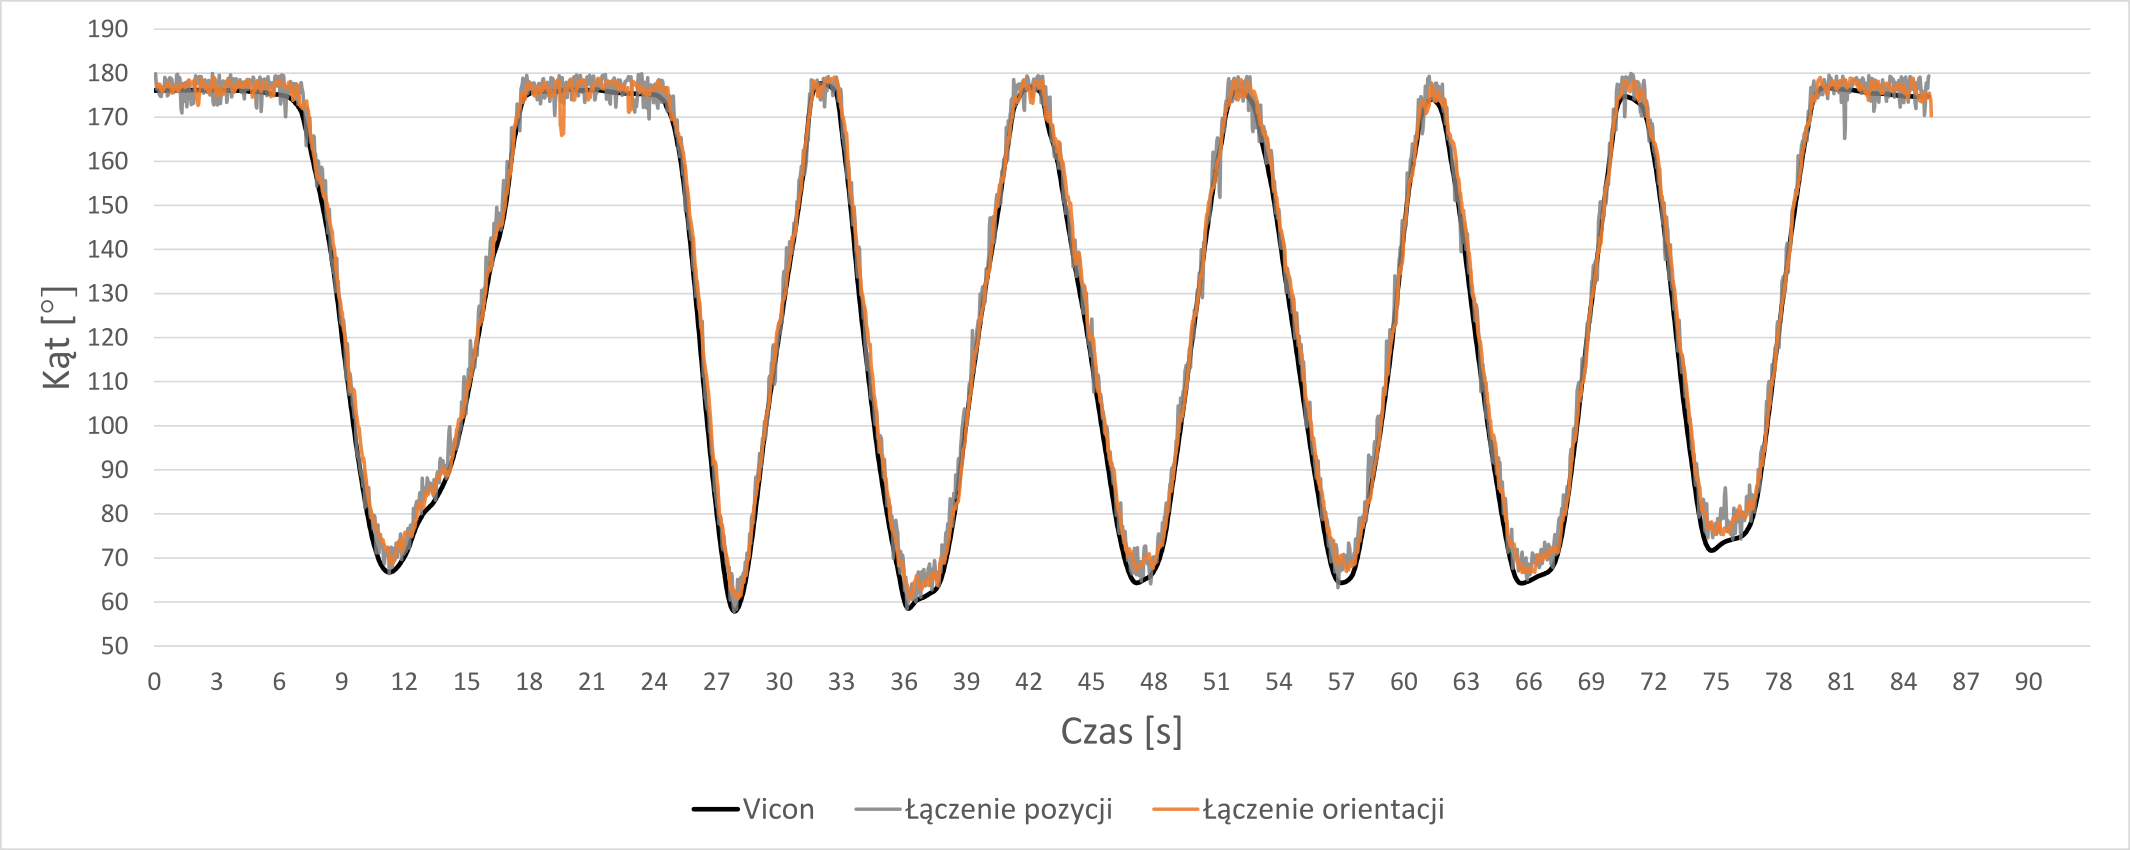
\includegraphics[width=0.9\linewidth]{images/200/angle.png}
		\caption{Wykres przedstawiający oszacowanie wartości kąta zgięcia ręki w łokciu ($\beta$) w trakcie ćwiczenia 2}
		\label{fig:experiments:second:angle}
	\end{figure}
\end{savenotes}
\begin{savenotes}
	\begin{figure}[!htb]
		\centering
		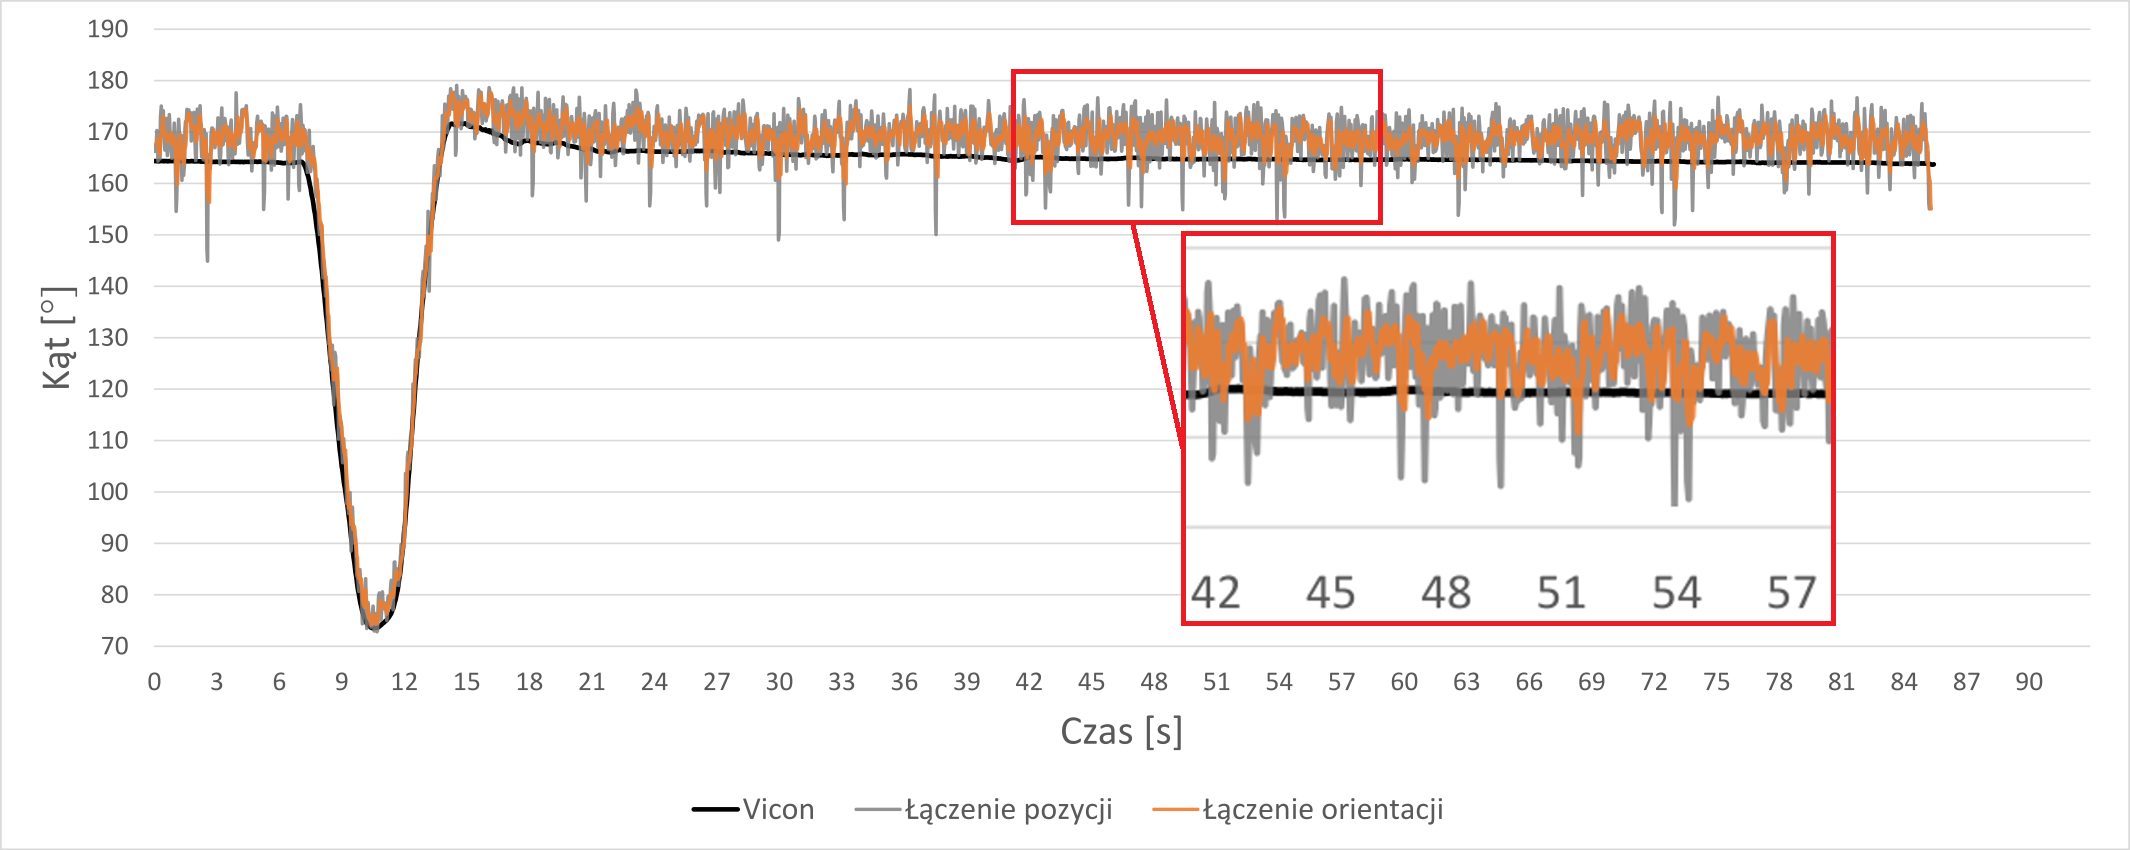
\includegraphics[width=0.9\linewidth]{images/300/angle.png}
		\caption{Wykres przedstawiający oszacowanie wartości kąta zgięcia ręki w łokciu ($\beta$) w trakcie ćwiczenia 3}
		\label{fig:experiments:third:angle}
	\end{figure}
\end{savenotes}
																				
\section*{Ćwiczenie 4 -- Utrzymanie wyprostowanych ramion}
Celem ostatniego ćwiczenia było sprawdzenie stabilności pomiarów w~przypadku długiego braku ruchu. W~tym wypadku urządzeniem, którego dane pomiarowe mogą szczególnie ulec pogorszeniu w~trakcie działania jest urządzenie zbudowane z~czujników inercyjnych. Tabela \ref{tab:experiments:four:avg} zawiera zestawienie dokładności pomiarów dla tego eksperymentu.
																				
\begin{table}[!htb]
	\caption[Średni błąd szacowania $\overline{RMSE}$ dla ćwiczenia nr 4]{Średni błąd szacowania $\overline{RMSE}$ (wz. \ref{eq:experiments:comparison}) dla ćwiczenia nr 4}
	\label{tab:experiments:four:avg}
	\noindent
	\tiny
	\centering
	\begin{tabular}{|c|N{1}{2}|N{1}{2}|N{1}{2}|N{1}{2}|N{1}{2}|N{1}{2}|}		
		\toprule 
		& \multicolumn{3}{c|}{{Metoda autorska}} & \multicolumn{3}{c|}{{Metoda Kalkbrennera}}  \\ 
		\midrule 
		{Sesja}                    & {$RMSE^O_E$} & {$RMSE^O_W$} & {$RMSE^O_\beta$} & {$RMSE^P_E$} & {$RMSE^P_W$} & {$RMSE^P_\beta$} \\
		{śledzenia}               & {$[cm]$}     & {$[cm]$}     & {$[\degree]$}    & {$[cm]$}     & {$[cm]$}     & {$[\degree]$}    \\	
		\midrule		
		1                          & 2.1208       & 2.3861       & 4.5450           & 2.3990       & 2.7321       & 4.8643           \\
		2                          & 2.2612       & 2.6185       & 3.8645           & 2.4400       & 2.7574       & 5.1007           \\
		3                          & 2.1646       & 2.4969       & 3.6962           & 2.5821       & 2.8521       & 4.2370           \\
		4                          & 2.3011       & 2.5810       & 4.2258           & 2.5777       & 2.8544       & 4.6130           \\
		5                          & 2.5827       & 2.4711       & 4.3170           & 2.4692       & 2.7876       & 4.8454           \\
		6                          & 2.1827       & 2.4813       & 4.0222           & 2.3609       & 2.7499       & 4.2690           \\
		\midrule
																																																																		
		Średnia $\overline{RMSE}$ & 2.2688       & 2.5058       & 4.1118           & 2.4715       & 2.7889       & 4.6549           \\
		Odchylenie                 & 0.1526       & 0.0758       & 0.2842           & 0.0836       & 0.0483       & 0.3173           \\
		\bottomrule
	\end{tabular} 
																																										
\end{table} 
																				
Podobnie jak w~ćwiczeniu 1, tak i~w~ćwiczeniu 4, oba urządzenia były w~stanie śledzić ruchy wykonywane przez śledzonego aktora przez cały czas trwania eksperymentu. Jednak, podobnie jak we wspomnianym ćwiczeniu, zmianie ulegały długości segmentów kości i~miało to przełożenie na działanie metody Kalkbrennera. Wizualizacje łańcuchów kinematycznych przedstawione na rysunku \ref{fig:experiments:four} pokazują, że Kinect, mimo pełnej widoczności całej ręki, miał trudność z~poprawnym określeniem jej pozycji w~osi pionowej. Mimo to obie metody były w~stanie wyznaczyć pozycje stawów z~lepszą dokładnością niż każde z~urządzeń pomiarowych osobno.
																				
\begin{savenotes}
	\begin{figure}[!htb]
		\captionsetup{singlelinecheck=off}
		\centering
		\begin{subfigure}[b]{0.9\textwidth}
			\centering
			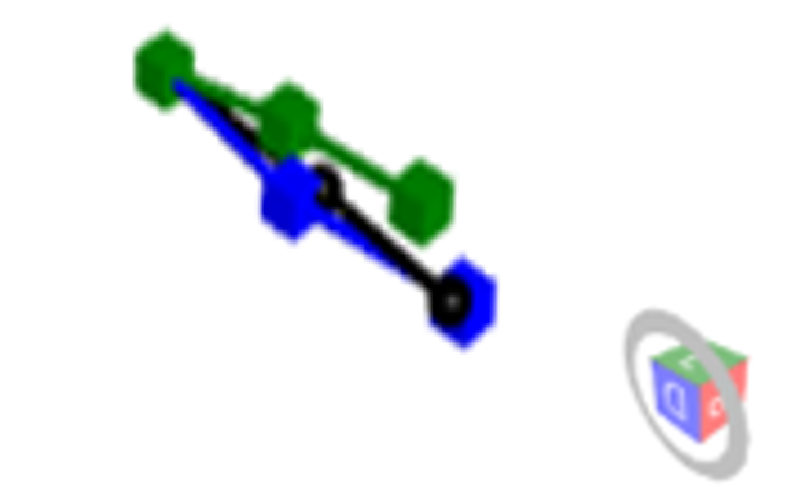
\includegraphics[width=\linewidth]{images/400/raw.png}	
			\caption{Wizualizacja ruchu bezpośrednio z~urządzeń pomiarowych}
			\label{fig:experiments:four:raw}
		\end{subfigure}
																																											
		\begin{subfigure}[b]{0.9\textwidth}
			\centering
			\includegraphics[width=\linewidth]{images/400/Fused.png}		
			\caption{Wizualizacja ruchu po złączeniu danych z~urządzeń pomiarowych}
			\label{fig:experiments:four:fused}	
		\end{subfigure}
																																										
		\caption[Wizualizacja ruchu ręki w~ćwiczeniu 4]{Wizualizacja ruchu ręki w~ćwiczeniu 4.  Kolory: czarny -- Vicon, niebieski -- czujniki inercyjne, zielony -- Kinect, szary -- metoda Kalkbrennera, pomarańczowy -- metoda autorska}	
		\label{fig:experiments:four}
	\end{figure}
\end{savenotes}
																						
Wykresy estymacji położenia stawu łokciowego (rys. \ref{fig:experiments:four:elbowZ}) oraz nadgarstkowego (rys. \ref{fig:experiments:four:wristZ}) pozwalają zaobserwować wpływ stabilności pomiarów jednego stawu na drugi. Jest to szczególnie widoczne w~wykresie metody Kalkbrennera, gdzie amplituda drgań pozycji nadgarstka jest widocznie większa niż w~przypadku drgań łokcia. 
																						
\begin{savenotes}
	\begin{figure}[!htb]
		\centering
		\begin{subfigure}[b]{0.9\textwidth}
			\centering
			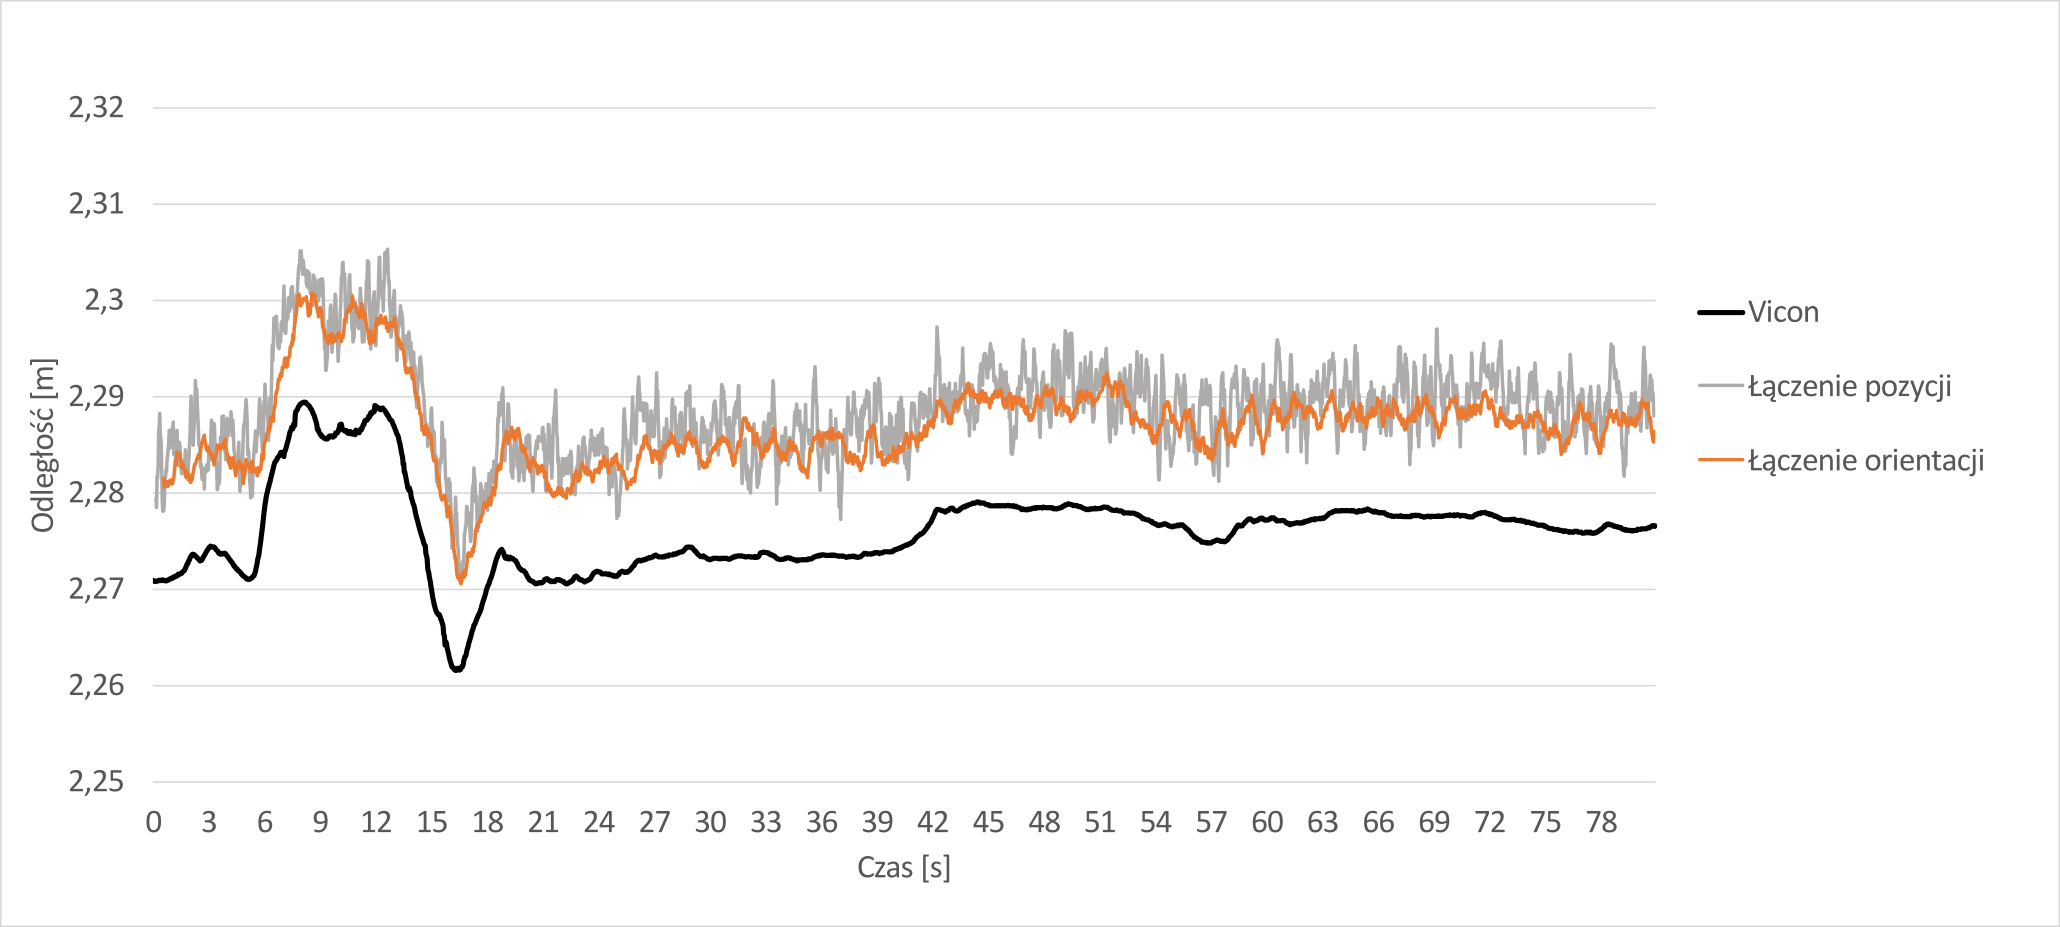
\includegraphics[width=\linewidth]{images/400/3.png}		
			\caption{Łokieć}
			\label{fig:experiments:four:elbowZ}
		\end{subfigure}
		\begin{subfigure}[b]{0.9\textwidth}
			\centering
			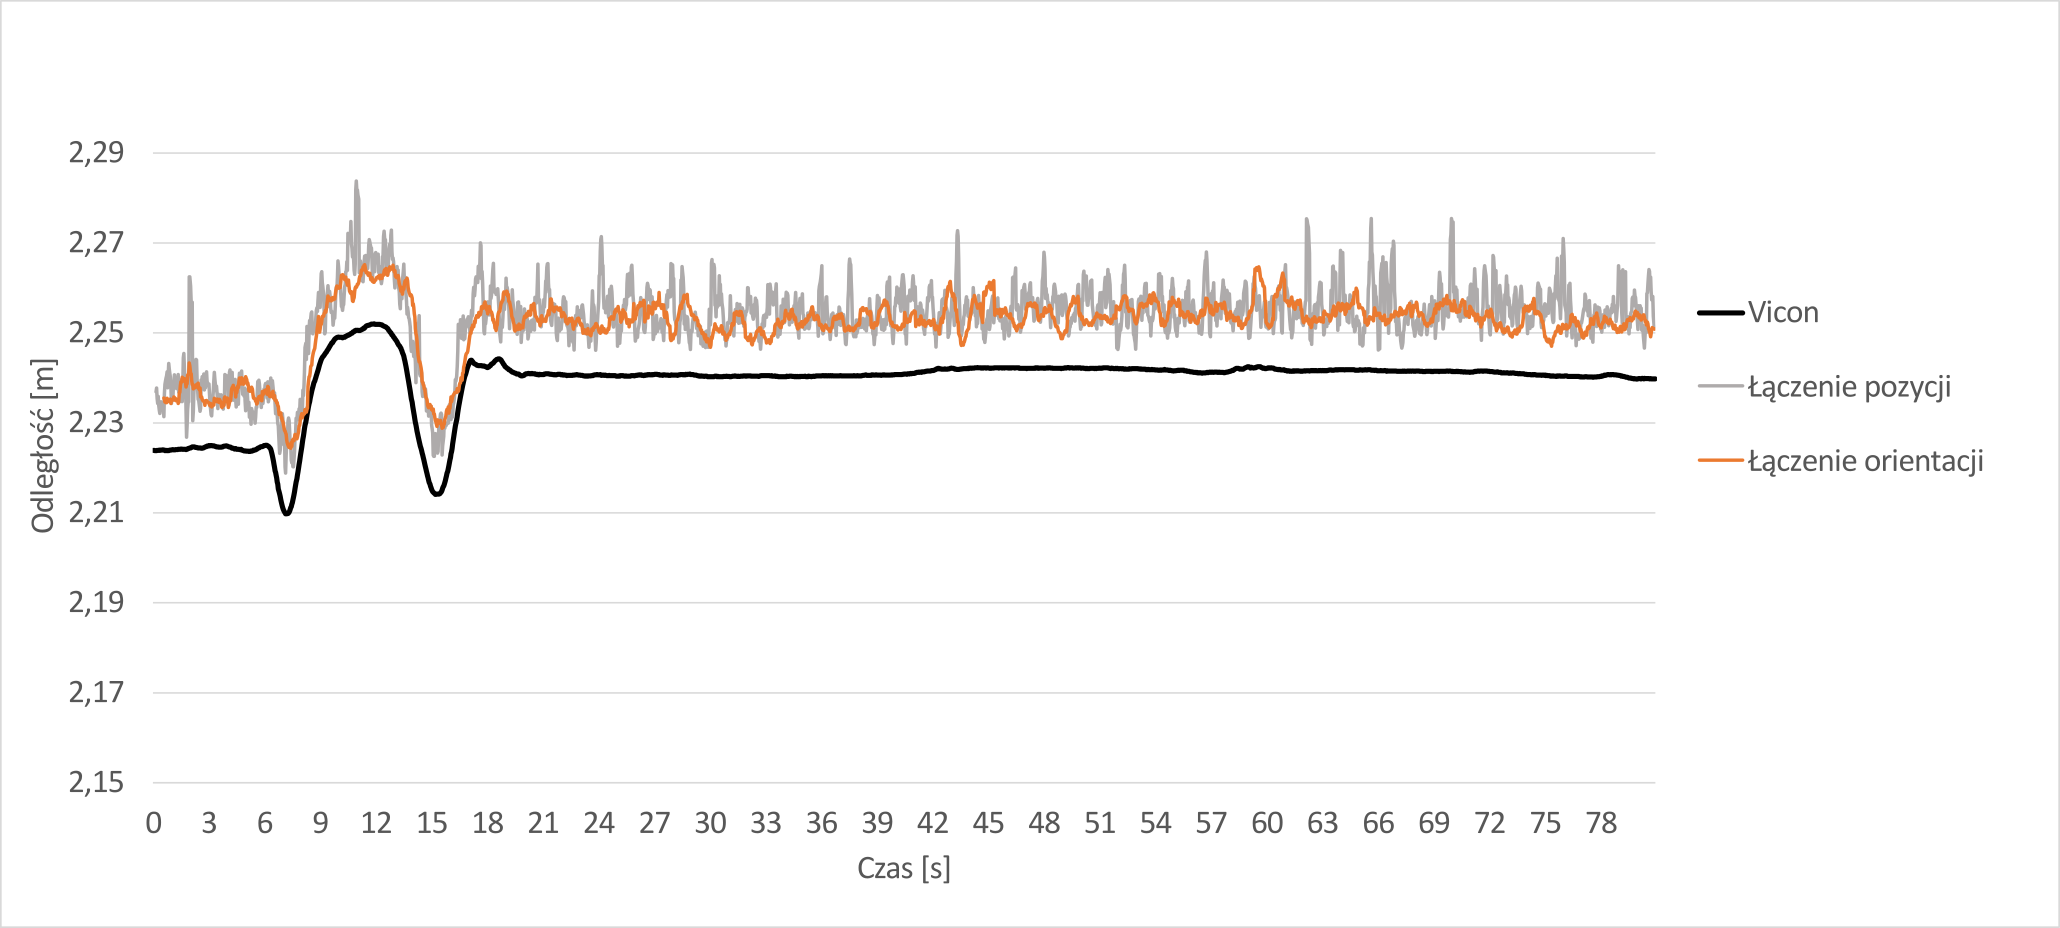
\includegraphics[width=\linewidth]{images/400/6.png}		
			\caption{Nadgarstek}
			\label{fig:experiments:four:wristZ}
		\end{subfigure}
		\caption[Wykres położenia stawu łokciowego i nadgarstkowego w~osi Z~w~ćwiczeniu 4]{Wykres położenia stawu łokciowego (a) i nadgarstkowego (b) w~osi Z~w~ćwiczeniu 4}	
		\label{fig:experiments:four:Zaxis}
	\end{figure}
\end{savenotes}
		
Wykres estymacji kąta $\beta$ w trakcie ćwiczenia 4 zaprezentowany na rysunku \ref{fig:experiments:fourth:angle} pozwala zauważyć podobne zachowanie do tego zaobserwowanego w~ćwiczeniu 1. W trakcie wykonywania ruchu (w tym ćwiczeniu zamierzona zmiana kąta w łokciu następowała tylko podczas początkowej synchronizacji) widać estymację kąta za pomocą obu metod zbliżoną do danych referencyjnych. Różnica jest natomiast dobrze widoczna podczas braku ruchu. Wówczas widoczne są wyraźne fluktuacje w~oszacowaniach wartości kąta które wpływają na wartość uzyskanego błędu średniowkadratowego.
			
\begin{savenotes}
		\begin{figure}[!htb]
			\centering
			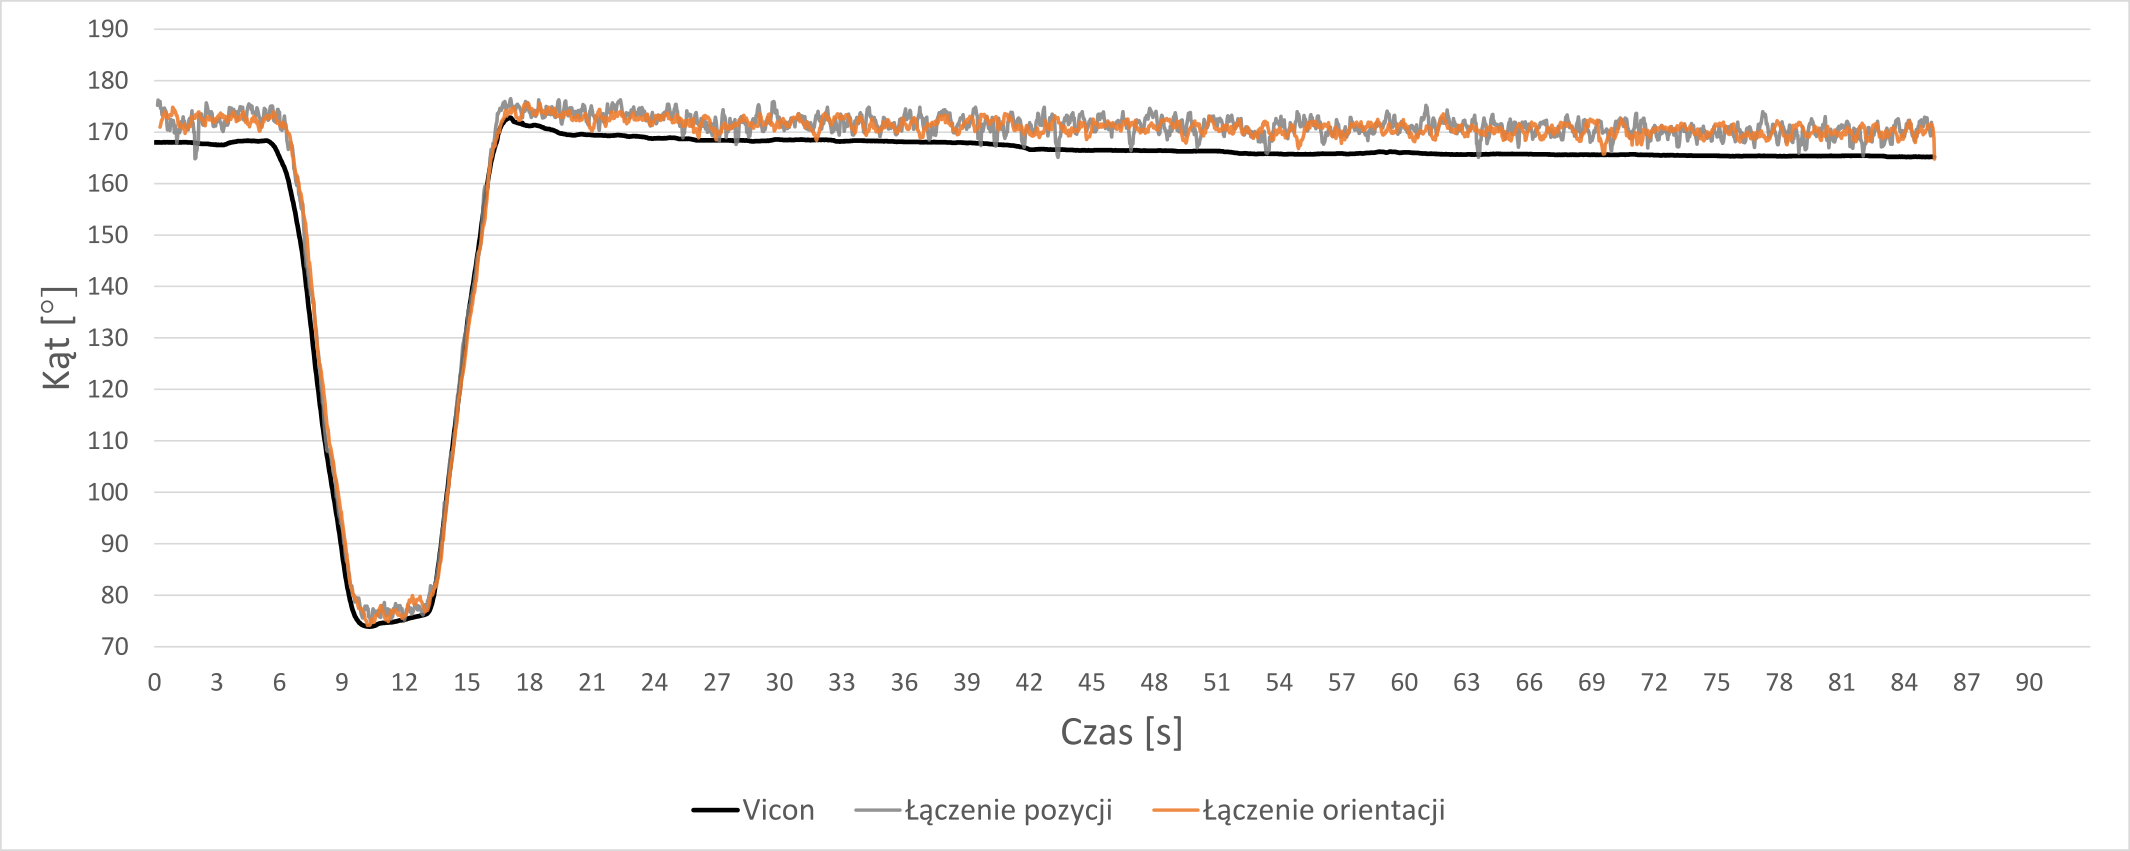
\includegraphics[width=0.9\linewidth]{images/400/angle.png}
			\caption{Wykres przedstawiający oszacowanie wartości kąta zgięcia ręki w łokciu ($\beta$) w trakcie ćwiczenia 4}
			\label{fig:experiments:fourth:angle}
		\end{figure}
\end{savenotes}																					
\section{Podsumowanie}
																								
Ćwiczenia wykonywane w~ramach eksperymentów miały za zadanie sprawdzić działanie metody autora niniejszej pracy, i porównać ją z metodą Kalkbrennera w~sytuacji, gdy jeden z~czujników przestaje być wiarygodny oraz kiedy otrzymywane dane są degradowane w~czasie. Dla kontrastu weryfikacja dokładności porównywanych metod, dokonana została także na bazie ćwiczenia, które dla obu urządzeń pomiarowych może być nazywane neutralnym (ćwiczenie 1).\\
																								
Porównane ze sobą zostały trzy wartości wyznaczone przez dwie metody: metodę Kalkbrennera i~metodę łączącą dane opartą o~obroty kości. Wartościami porównywanymi były: położenie stawu łokciowego, położenie stawu nadgarstkowego oraz kąt zgięcia ręki w~łokciu ($\beta$). Błąd oszacowania pozycji stawów w~przestrzeni (wz. \ref{eq:experiments:average}) może być wykorzystany jako wskaźnik na ile dana metoda mogłaby być wykorzystana tam gdzie istotne może być wykrycie czy dochodzi do interakcji pomiędzy estymowanym modelem a~otoczeniem. Jako przykład można podać środowisko wirtualne, w~którym znajdują się obiekty którymi można manipulować. Każdy taki obiekt ma swoje ściśle określone położenie w~przestrzeni, a~estymacja pozycji stawów jest niezędna żeby określić czy doszło już do interakcji z~takim obiektem czy nie.
																								 
Trzecia wartość -- kąt zgięcia ręki w~łokciu ($\beta$) -- jest uniezależniona od przyjętych długości kości i~ewentualnych błędów w~pomiarach tych długości. Określa ona wzajemną orientację pomiędzy kością przedramienia a~ramieniem w~zakresie stopnia swobody stawu łokciowego. Ona też pozwala na zweryfikowanie badanych metod śledzenia na potrzeby kontroli zakresu ruchu stawu łokciowego, co może być przydatne w~procesie rehabilitacji ruchowej. \\ 

\begin{savenotes}
	\begin{figure}[!htb]
		\centering
		\begin{tikzpicture}
			\begin{axis}[
					ybar,
					bar width=.5cm,
					width=\textwidth,
					height=.5\textwidth,
					legend style={at={(0.5,1)},
						anchor=north,legend columns=-1},
					symbolic x coords={ex 1,ex 2,ex 3,ex 4},
					xticklabels={Ćwiczenie 1,Ćwiczenie 2,Ćwiczenie 3,Ćwiczenie 4},
					xtick=data,
					ymin=0,ymax=5,
					ylabel={$\overline{RMSE} [cm]$},
				]
				\addplot [black,fill=white,error bars/.cd,y dir=both,y explicit] coordinates { 
					(ex 1,2.6) +- (0.0, 0.07)         
					(ex 2,3.1) +- (0.0, 0.11)
					(ex 3,2.9) +- (0.0, 0.18)  
				(ex 4,2.5) +- (0.0, 0.08) };
				\addplot [black,fill=gray80,error bars/.cd,y dir=both,y explicit] coordinates { 
					(ex 1,2.2) +- (0.0, 0.08)         
					(ex 2,2.5) +- (0.0, 0.14)
					(ex 3,2.5) +- (0.0, 0.23)  
				(ex 4,2.3) +- (0.0, 0.16) };
				\legend{Metoda Kalkbrennera, Metoda autorska}
				\node at (axis cs:ex 1,4){\textcolor{black}{r = 13\%}};
				\node at (axis cs:ex 2,4){\textcolor{black}{r = 18\%}};
				\node at (axis cs:ex 3,4){\textcolor{black}{r = 14\%}};
				\node at (axis cs:ex 4,4){\textcolor{black}{r = 7\%}};
			\end{axis}
		\end{tikzpicture}	
		\caption{Średni błąd średniokwadratowy wyznaczania pozycji łokcia}
		\label{fig:experiments:elbow:summary}
	\end{figure}
\end{savenotes}
																										
\begin{savenotes}
	\begin{figure}[!htb]
		\centering
		\begin{tikzpicture}
			\begin{axis}[
					ybar,
					bar width=.5cm,
					width=\textwidth,
					height=.5\textwidth,
					legend style={at={(0.5,1)},
						anchor=north,legend columns=-1},
					symbolic x coords={ex 1,ex 2,ex 3,ex 4},
					xtick=data,
					ymin=0,ymax=5,
					xticklabels={Ćwiczenie 1,Ćwiczenie 2,Ćwiczenie 3,Ćwiczenie 4},
					ylabel={$\overline{RMSE} [cm]$},
				]
				\addplot [black,fill=white,error bars/.cd,y dir=both,y explicit] coordinates { 
					(ex 1,3.0) +- (0.0, 0.05)
					(ex 2,3.4) +- (0.0, 0.1)
					(ex 3,3.3) +- (0.0, 0.24)
				(ex 4,2.8) +- (0.0, 0.04)};
				\addplot [black,fill=gray80,error bars/.cd,y dir=both,y explicit] coordinates { 
					(ex 1,2.9) +- (0.0, 0.07)
					(ex 2,2.9) +- (0.0, 0.12)
					(ex 3,2.8) +- (0.0, 0.2)
				(ex 4,2.5) +- (0.0, 0.07)};
																																																																																																					
				\legend{Metoda Kalkbrennera, Metoda autorska}
				\node at (axis cs:ex 1,4){\textcolor{black}{r = 8\%}};
				\node at (axis cs:ex 2,4){\textcolor{black}{r = 16\%}};
				\node at (axis cs:ex 3,4){\textcolor{black}{r = 14\%}};
				\node at (axis cs:ex 4,4){\textcolor{black}{r = 9\%}};
			\end{axis}
		\end{tikzpicture}
		\caption{Średni błąd średniokwadratowy wyznaczania pozycji nadgarstka}
		\label{fig:experiments:wrist:summary}
	\end{figure}
\end{savenotes}

Wykresy z~rysunków \ref{fig:experiments:elbow:summary}, \ref{fig:experiments:wrist:summary} oraz \ref{fig:experiments:angle:summary} pokazują podsumowanie porównania uśrednionych wartości błędu uzyskanych oszacowań ($\overline{RMSE}$) za pomocą metody Kalkbrennera oraz metody autora tej pracy.
%([TODO] teraz czuje, że metoda powinna mieć jakiś skrót, np. od angielskiej jej nazwy, którą pewnie trzeba wymyśleć - Oriented-based Hybrid Motion Tracking -> OHMT => najbliżej jest MOTH tylko jak? / Jest jeszcze HOMT -> Hybrid, Oriented-based Motion Tracking tylko ten skrótowiec występuje też w~slangu: http://www.urbandictionary.com/define.php?term=H.O.M.T. ). 
Widać na~nich poprawę w~wyznaczaniu położenia stawu łokciowego do 18\%, nadgarstowego do 16\% oraz zdolności szacowania kąta zgięcia ręki w~łokciu do 11\%. Z~przedstawionych wyników wynika większa poprawa w~wyznaczaniu pozycji łokcia niż w~przypadku nadgarstka. Spowodowane jest to kumulowaniem się błędów własnych estymacji położenia nadgarstka, jak i~błędów estymacji położenia łokcia. Jest to cecha charakterystyczna stosowania hierarchicznego modelu ciała człowieka. Dla przyjętej hierarchicznej reprezentacji układu kostnego postaci, czym badany staw jest bardziej odległy od punktu początkowego (korzenia) tym dokładność estymacji jego położenia jest mniejsza i~mniejsze są możliwości jej poprawy.\\

																															
\begin{savenotes}
	\begin{figure}[!htb]
		\centering
		\begin{tikzpicture}
			\begin{axis}[
					ybar,
					bar width=.5cm,
					width=\textwidth,
					height=.5\textwidth,
					legend style={at={(0.5,1)},
						anchor=north,legend columns=-1},
					symbolic x coords={ex 1,ex 2,ex 3,ex 4},
					xtick=data,
					xticklabels={Ćwiczenie 1,Ćwiczenie 2,Ćwiczenie 3,Ćwiczenie 4},
					ymin=0,ymax=20,
					ylabel={$\overline{RMSE} [\degree]$},
				]
				\addplot [black,fill=white,error bars/.cd,y dir=both,y explicit] coordinates { 
					(ex 1,3.54) +- (0.0, 0.12)
					(ex 2,14.49) +- (0.0, 0.77)
					(ex 3,14.71) +- (0.0, 1.57)
					(ex 4,4.65)  +- (0.0, 0.32)
				};
				\addplot [black,fill=gray80,error bars/.cd,y dir=both,y explicit] coordinates { 
					(ex 1,3.29) +- (0.0, 0.12)
					(ex 2,13.35)+- (0.0, 0.65)
					(ex 3,14.08)+- (0.0, 1.55)
				(ex 4,4.11)  +- (0.0, 0.29)};
																																																																																																							
				\legend{Metoda Kalkbrennera, Metoda autorska}
				\node at (axis cs:ex 1,16){\textcolor{black}{r = 6\%}};
				\node at (axis cs:ex 2,16){\textcolor{black}{r = 8\%}};
				\node at (axis cs:ex 3,16){\textcolor{black}{r = 4\%}};
				\node at (axis cs:ex 4,16){\textcolor{black}{r = 11\%}};
			\end{axis}
		\end{tikzpicture}	
		\caption{Średni błąd średniokwadratowy wyznaczania kąta zgięcia ręki w~łokciu $\beta$}
		\label{fig:experiments:angle:summary}
	\end{figure}
\end{savenotes}


Również na wykresie z~rysunku \ref{fig:experiments:angle:summary}, reprezentującym wyniki szacowania kąta zgięcia ręki w~łokciu za pomocą obu metod, widać zmniejszenie błędu wyników uzyskiwanych przez metodę opisywaną w niniejszej dysertacji. Sugeruje to, że łącząc ze sobą informacje o orientacji kości, możliwe jest dokładniejsze odtworzenie pozy, w jakiej znajduje się śledzona postać, niż ma to miejsce w przypadku łączenia informacji o pozycjach stawów. Precyzyjne oszacowanie wzajemnej orientacji pomiędzy poszczególnymi kośćmi, z jednoczesnym wykorzystaniem modelu szkieletowego o stałych wartościach długości poszczególnych segmentów, ma bezpośrednie przełożenie na wielkość uzyskiwanego błędu. Można przyjąć, że kombinacja tych dwóch cech: łączenie ze sobą informacji o obrotach kości oraz definicja długości kości zakładająca niezmienność tych wartości, mają decydujący wpływ na błąd szacowania pozycji stawów. Jednocześnie, poprawienie szacowania wartości kąta zgięcia ręki wpływa na zmniejszenie ilości występujących drgań poszczególnych segmentów modelu szkieletowego wyznaczonego przez metodę autora tej pracy.